\documentclass[titlepage]{article}


% ==================== BASIC FORMATTING ====================
\setlength{\parindent}{0pt} % removes indents from paragraphs
\setlength{\parskip}{3pt}   % adds small space between paragraphs
% ==========================================================


% ==================== PACKAGES ====================
\usepackage{cancel} % allows striking out of text
\usepackage{xfrac} % diagonal fraction
\usepackage{float}
\usepackage{amsfonts,amssymb,amsmath,latexsym,amsthm,mathrsfs,cases} % basic [mathabx] math symbols
\usepackage{tikz}
\usetikzlibrary{arrows,automata,positioning}
\usepackage{graphicx}  % add graphics by \includegraphics
\usepackage[margin=1in]{geometry}
\usepackage{arydshln}
\usepackage{etoolbox}
\usepackage{color}
\usepackage{listings} % to add python/MATLAB code
\usepackage[final, nopatch=footnote]{microtype} % microtype
\usepackage{enumerate}
\usepackage[shortlabels]{enumitem}
\usepackage{empheq} % To use left bracket and subequations at the same time
\usepackage{titlesec}
\usepackage{subcaption}
\usepackage{caption}
\usepackage{listings} % For creating listing environments/ code boxes
\usepackage{xcolor} % Optional: for custom colors
\usepackage{pdfpages} % connect a pdf to your latex document with this
\usepackage[most]{tcolorbox} % Adds boxes into latex to emphasize different content
\usepackage{graphicx}
\usepackage{titlepic}
% =========================================================



% ==================== CODE BOXES SETUP ====================
\lstset{
    basicstyle=\footnotesize\ttfamily,
    commentstyle=\color{green!60!black},
    keywordstyle=\color{blue},
    stringstyle=\color{purple},
    breaklines=true,
    captionpos=b, % Caption position at the bottom
    % Add other desired styles
}
% =========================================================


% ==================== TEXT BOXES SETUP ====================

\newtcolorbox{myboxg}{
  breakable,
  colback=blue!5!white,
  colframe=blue!75!black
}
% ==========================================================


% ==================== TEXT BOXES SETUP ====================

\newtcolorbox{myboxr}{
  breakable,
  colback=red!5!white,
  colframe=red!75!black
}
% ==========================================================


% ==================== HYPERLINK SETUP ====================
\usepackage[hidelinks]{hyperref}  %% add box and hyperlinks to equation numbers
\definecolor{darkblue}{rgb}{0.0,0.0,0.3}
\hypersetup{colorlinks,breaklinks,
            linkcolor=blue,urlcolor=blue,
            anchorcolor=darkblue,citecolor=darkblue}
% =========================================================


% ==================== SECTION TITLES ====================
\titleformat{\section}[block]
  {\normalfont\large\bfseries}{Section \thesection:}{5pt}{}
\titleformat{name=\section,numberless}[block]
  {\normalfont\large\bfseries}{}{0pt}{}
% ========================================================


% ==================== HOMEWORK AND EXAM PRACTICE HEADERS ====================
% Define a new counter for homework
\newcounter{homework}
\renewcommand{\thehomework}{\arabic{homework}}
\newcommand{\homework}[1]{%
  \refstepcounter{homework}%
  \section*{Homework \thehomework: #1}%
  \addcontentsline{toc}{section}{Homework \thehomework: #1}%
} 
% Define a new counter for Exam Practice
\newcounter{exampractice} % Define counter
\renewcommand{\theexampractice}{\arabic{exampractice}}
\newcommand{\exampractice}[1]{%
  \refstepcounter{exampractice}%
  \section*{Exam Practice \theexampractice: #1}%
  \addcontentsline{toc}{section}{Exam Practice \theexampractice: #1}%
}
% ============================================================================


% ==================== THEOREM ENVIRONMENTS ====================
\theoremstyle{plain}
\newtheorem{theorem}{Theorem}[section]
\newtheorem{lemma}[theorem]{Lemma}
\newtheorem{proposition}[theorem]{Proposition}
\newtheorem{corollary}[theorem]{Corollary}
\newtheorem{acknowledgement}[theorem]{Acknowledgement}
\newtheorem{algorithm}[theorem]{Algorithm}
\newtheorem{axiom}[theorem]{Axiom}
\newtheorem{case}[theorem]{Case}
\newtheorem{claim}[theorem]{Claim}
\newtheorem{conclusion}[theorem]{Conclusion}
\newtheorem{condition}[theorem]{Condition}
\newtheorem{conjecture}[theorem]{Conjecture}
\newtheorem{criterion}[theorem]{Criterion}
\newtheorem{notation}[theorem]{Notation}
\newtheorem{problem}[theorem]{Problem}
\newtheorem{summary}[theorem]{Summary}

\theoremstyle{definition}
\newtheorem{definition}{Definition}[section]
\newtheorem{result}{Result}[section]

\theoremstyle{remark}
\newtheorem{remark}{Remark}[section]
\newtheorem{bfremark}[remark]{\bf Remark}
\newtheorem{example}[remark]{Example}
\newtheorem{question}{\bf Question}[section]
\newtheorem{note}{Note}

\newtheoremstyle{exercise-style}% name
  {\topsep}% space above
  {\topsep}% space below
  {}% body font
  {}% indent amount
  {\itshape}% theorem head font
  {}% punctuation after theorem head
  {.5em}% space after theorem head
  {\thmname{#1}\thmnumber{ #2}\thmnote{ (#3)}.}% theorem head spec
\theoremstyle{exercise-style}
\newtheorem{exercise}{Exercise}[section]
\newtheorem{PCexercise}[exercise]{PC-Exercise}
% ==============================================================


% ==================== NUMBERING ====================
\numberwithin{equation}{section}
\numberwithin{theorem}{section}
\numberwithin{remark}{section}
% ===================================================


%%%%%%%% new syntax by Xiang Wan %%%%%%%%%
\newcommand{\inner}[1]{{\left\langle #1 \right\rangle}}
\newcommand{\norm}[1]{{\left\| #1 \right\|}}
\newcommand{\B}[1]{{\bf #1}}
\newcommand{\BB}[1]{{\mathbb #1}}
\newcommand{\CAL}[1]{{\mathcal #1}}
\newcommand{\inv}[1]{{#1^{-1}}}
\newcommand{\BC}{\mathbb{C}}
\newcommand{\BN}{\mathbb{N}}
\newcommand{\BP}{\mathbb{P}}
\newcommand{\BQ}{\mathbb{Q}}
\newcommand{\BR}{\mathbb{R}}
\newcommand{\BZ}{\mathbb{Z}}
\newcommand{\ds}{\displaystyle}
\newcommand{\lt}{<}
\newcommand{\normm}[2]{\left \lVert #1 \right \rVert_{#2}}
\newcommand{\HRule}[1]{\rule{\linewidth}{#1}}

%%%%%%%%%%%%%%%%%%%%%%%%%%%%%%%%%%%%%%%%%%%%%%%%%%%%%%%%%%%%%%%%%%%%%%%%%
%%%%%%%%%%%%%%%%%%%%% Do not change the lines above %%%%%%%%%%%%%%%%%%%%%
%%%%%%%%%%%%%%%%%%%%%%%%%%%%%%%%%%%%%%%%%%%%%%%%%%%%%%%%%%%%%%%%%%%%%%%%%


% ------------------------------------------------------------------------------
\title{Representation Theory Final Exam Study Guide}
\author{Will Bales \& Delaney Rager \& Ramsay Barlow}
\date{\today}
\titlepic{
\includegraphics[width=0.5\textwidth]{pictures/images.jpg}}

\begin{document}

\maketitle

\tableofcontents

\section{Things to Study}

\begin{myboxr}
    \begin{note}[Final Exam Contents According to Sakai]
        The contents of the final exam will follow these topics:
        \begin{enumerate}
            \item Group Actions
            \item Classification of Permutation Representations
            \item Burnside's Lemma
            \item Lectures 1-6 of Representation Theory (Definitions, Examples, Propositions, Lemmas, Corollaries) 
            \item Lecture 3: Thm 4.1
            \item Lecture 4: Prop 2.6, Thm 3.2 (please read this proof, but it is not included in the final).
            \item Lecture 5: Prop 1.1, Prop 3.2, Prop 4.1.(i)
            \item Lecture 6: Prop 2.3, Prop 2.6, Cor 2.7, Thm 5.1
            \item HWK 3
            \item Previous two exams (I will choose at least one problem from one of the previous midterms) (TEST 1 AND TEST 2)
        \end{enumerate}
    \end{note}
\end{myboxr}

\section{Final Exam Review}

\subsection{Theorems and Proofs of Theorems}

\begin{myboxg}
    \begin{theorem}[Theorem L3-4.1: Irreducible representations of abelian groups]
        Let $G$ be a finite abelian group and $V$ an irreducible representation of $G$ over $\mathbb{C}$. Then
        \begin{align}
        \dim V = 1.
        \end{align}
    \end{theorem}
\end{myboxg}

\begin{proof}
    Let $\rho : G \to \mathrm{GL}(V)$ be an irreducible representation and let $h \in G$. Then $\rho(h) : V \to V$ is a linear isomorphism. We claim $\rho(h)$ is a $G$-module homomorphism.
    
    Indeed, for all $g \in G$ and $v \in V$:
    \begin{align}
        \rho(h)(\rho(g)(v)) &= \rho(hg)(v) \\
        &= \rho(gh)(v) \\
        &= \rho(g)(\rho(h)(v)),
    \end{align}
    where the middle equality uses the fact that $G$ is abelian.
    
    So $\rho(h)$ is a $G$-endomorphism of the irreducible module $V$.
    
    By Schur’s Lemma (ii), 
    \begin{align}
        \rho(h) = \lambda_h \cdot \mathrm{id}_V
    \end{align}
    for some $\lambda_h \in \mathbb{C}$ (with $\lambda_h \neq 0$ since $\rho(h)$ is invertible).
    
    Now fix any nonzero $w \in V$. For every $g \in G$,
    \begin{align}
        g \cdot w = \lambda_g w \in \mathbb{C}\{w\}.
    \end{align}
    
    So $W = \mathbb{C}\{w\}$ is a one-dimensional $G$-submodule of $V$. Since $V$ is irreducible and $W \neq \{0\}$, we get $V = W$, i.e.
    \begin{align}
        \dim V = 1.
    \end{align}
\end{proof}

\begin{myboxg}
    \begin{proposition}[Proposition L4-2.6: Orthogonal complements of $G$-submodules]
        Let $V$ be a $G$-module with a $G$-invariant inner product $\langle \cdot, \cdot \rangle$, and let $W \subseteq V$ be a $G$-submodule. Then $W^\perp$ is also a $G$-submodule, and consequently
        \begin{align}
            V = W \oplus_G W^\perp.
        \end{align}
    \end{proposition}
\end{myboxg}

\begin{proof}
    Let $u \in W^\perp$ and $g \in G$. We must show $g \cdot u \in W^\perp$, i.e., that $\langle g \cdot u, w \rangle = 0$ for all $w \in W$.
    
    Since $W$ is a $G$-submodule, $g^{-1} \cdot w \in W$ for all $w \in W$. Using $G$-invariance of the inner product:
    \begin{align}
        \langle g \cdot u, w \rangle &= \langle g^{-1} \cdot (g \cdot u), g^{-1} \cdot w \rangle \\
        &= \langle u, g^{-1} \cdot w \rangle \\
        &= 0,
    \end{align}
    where the last equality holds because $u \in W^\perp$ and $g^{-1} \cdot w \in W$.
    
    Therefore $g \cdot u \in W^\perp$.
    
    Since $W^\perp$ is a $G$-submodule and $W \cap W^\perp = \{0\}$, we have
    \begin{align}
        V = W \oplus W^\perp,
    \end{align}
    a decomposition as $G$-modules.
\end{proof}

\begin{myboxg}
    \begin{theorem}[Theorem L4-3.2 Maschke’s Theorem - ONLY READ THROUGH (WILL NOT BE ON EXAM)]
    Let $G$ be a finite group and $V$ a finitely generated $\mathbb{C}G$-module (i.e., a finite-dimensional representation of $G$ over $\mathbb{C}$). Then:
    \begin{align}
        \text{(i)} \quad & \text{Every $G$-submodule of $V$ has a $G$-complement.} \\
        \text{(ii)} \quad & V = W^{(1)} \oplus_G W^{(2)} \oplus_G \cdots \oplus_G W^{(k)},
    \end{align}
    where each $W^{(i)}$ is an irreducible $G$-module.
    \end{theorem}
\end{myboxg}

\begin{proof}
    Before proving the theorem, we show that finiteness of $G$ is essential.
    
    \textbf{Example.} Let $G = (\mathbb{R}_{>0}, \cdot, 1)$ and define $\rho : G \to \mathrm{GL}_2(\mathbb{C})$ by
    \begin{align}
        \rho(r) =
        \begin{pmatrix}
        1 & \log r \\
        0 & 1
        \end{pmatrix}.
        \end{align}
        For $r,s \in G$,
        \begin{align}
        \rho(r)\rho(s)
        &=
        \begin{pmatrix}
        1 & \log r \\
        0 & 1
        \end{pmatrix}
        \begin{pmatrix}
        1 & \log s \\
        0 & 1
        \end{pmatrix} \\
        &=
        \begin{pmatrix}
        1 & \log r + \log s \\
        0 & 1
        \end{pmatrix} \\
        &=
        \begin{pmatrix}
        1 & \log(rs) \\
        0 & 1
        \end{pmatrix}
        = \rho(rs).
    \end{align}
    
    Let $W = \mathbb{C}\{e_1\}$. Then $W$ is $G$-invariant since $\rho(r)e_1 = e_1$.
    
    Suppose $U = \mathbb{C}\begin{pmatrix} a \\ b \end{pmatrix}$ is a $G$-complement with $b \neq 0$. Then invariance requires
    \begin{align}
        \rho(r)
        \begin{pmatrix}
        a \\ b
        \end{pmatrix}
        =
        \begin{pmatrix}
        a + b \log r \\
        b
        \end{pmatrix}
        \in U,
    \end{align}
    forcing
    \begin{align}
        \frac{a + b \log r}{b} = \frac{a}{b},
    \end{align}
    so $\log r = 0$ for all $r$, a contradiction.
    
    \medskip
    
    \textbf{(i)} Let $W \subseteq V$ be a $G$-submodule. Choose a basis $\{v_1,\dots,v_n\}$ of $V$ and define
    \begin{align}
        \langle v_i, v_j \rangle = \delta_{ij}.
    \end{align}
    
    Define a new form
    \begin{align}
        \langle u, v \rangle' = \sum_{g \in G} \langle g \cdot u, g \cdot v \rangle.
    \end{align}
    
    This is a Hermitian inner product: linearity and conjugate symmetry follow termwise, and
    \begin{align}
        \langle u, u \rangle' = \sum_{g \in G} \langle g \cdot u, g \cdot u \rangle \ge 0,
    \end{align}
    with equality only if $u = 0$.
    
    It is $G$-invariant since for $h \in G$,
    \begin{align}
        \langle h \cdot u, h \cdot v \rangle'
        &= \sum_{g \in G} \langle g h \cdot u, g h \cdot v \rangle \\
        &= \sum_{g' \in G} \langle g' \cdot u, g' \cdot v \rangle \\
        &= \langle u, v \rangle'.
    \end{align}
    
    Thus $W^\perp$ is a $G$-submodule and
    \begin{align}
        V = W \oplus W^\perp.
    \end{align}
    
    \medskip
    
    \textbf{(ii)} We proceed by induction on $\dim V$.
    
    If $\dim V = 1$, then $V$ is irreducible.
    
    If $V$ is reducible, there exists $0 \subsetneq W \subsetneq V$. By (i),
    \begin{align}
        V = W \oplus W'.
    \end{align}
    
    Since $\dim W, \dim W' < \dim V$, both decompose into irreducibles. Combining gives
    \begin{align}
        V = W^{(1)} \oplus_G \cdots \oplus_G W^{(k)}.
    \end{align}
\end{proof}

\begin{myboxg}
    \begin{proposition}[Proposition L5-1.1: One-dimensional representations of $\mathbb{Z}_n$]
        Let $\mathbb{Z}_n = \langle g \rangle$ be the cyclic group of order $n$ and let $\rho : \mathbb{Z}_n \to \mathrm{GL}_1(\mathbb{C})$ be a representation. Then
        \begin{align}
            \rho(g) = e^{2\pi i q / n}
        \end{align}
        for some $q \in \{0,1,\dots,n-1\}$.
        
        In particular, there are exactly $n$ one-dimensional representations of $\mathbb{Z}_n$, given by
        \begin{align}
            \rho_q(g) = e^{2\pi i q / n}, \quad q = 0,1,\dots,n-1.
        \end{align}
    \end{proposition}
\end{myboxg}

\begin{proof}
    Since $g^n = e$ and $\rho$ is a homomorphism, we have
    \begin{align}
        \rho(g)^n = \rho(g^n) = \rho(e) = 1.
    \end{align}
    
    So $\rho(g)$ is an $n$-th root of unity in $\mathbb{C}^\times$. The $n$-th roots of unity are precisely
    \begin{align}
        e^{2\pi i q / n}, \quad q = 0,1,\dots,n-1.
    \end{align}
    
    Each choice of $q$ determines a unique homomorphism $\rho_q : \mathbb{Z}_n \to \mathrm{GL}_1(\mathbb{C})$ via
    \begin{align}
        \rho_q(g^k) = e^{2\pi i qk / n}.
    \end{align}
    
    One easily verifies that $\rho_q$ is indeed a group homomorphism.
\end{proof}

\begin{myboxg}
    \begin{proposition}[Proposition L5-3.2: Isomorphic modules have the same character]
        If $V \cong W$ as $G$-modules, then
        \begin{align}
            \chi^V = \chi^W.
        \end{align}
    \end{proposition}
\end{myboxg}

\begin{proof}
    Let $\phi : V \to W$ be a $G$-module isomorphism. Then there exist bases $B_V$ of $V$ and $B_W$ of $W$ such that
    \begin{align}
        M_{B_V}(g) = M_{B_W}(g)
    \end{align}
    for all $g \in G$.
    
    Indeed, if $B_V = \{v_1,\dots,v_n\}$, take
    \begin{align}
        B_W = \{\phi(v_1),\dots,\phi(v_n)\}.
    \end{align}
    
    Therefore, for all $g \in G$,
    \begin{align}
        \chi_V(g) = \operatorname{Tr}(M_{B_V}(g)) = \operatorname{Tr}(M_{B_W}(g)) = \chi_W(g).
    \end{align}
\end{proof}

\begin{remark}[Observation]
    Characters are \textbf{not} group homomorphisms in general. That is, $\chi^V(gh) \neq \chi^V(g) \cdot \chi^V(h)$ in general, because $\mathrm{Tr}(AB) \neq \mathrm{Tr}(A)\mathrm{Tr}(B)$ in general.
\end{remark}

\begin{myboxg}
    \begin{proposition}[Proposition L5-4.1: Fundamental properties of characters (ONLY NEED TO KNOW (i))]
        Let $V$ be a $G$-module of dimension $n$ with character $\chi = \chi_V$. Then:
        \begin{align}
            \text{(i)} \quad & \chi(g^{-1}) = \chi(g) \quad \text{for all } g \in G, \\
            \text{(ii)} \quad & |\chi(g)| \le n \quad \text{for all } g \in G,
        \end{align}
        with equality in (ii) if and only if
        \begin{align}
            \rho(g) = \lambda \cdot \mathrm{id}_V
        \end{align}
        for some $\lambda \in \mathbb{C}$.
    \end{proposition}
\end{myboxg}

\begin{proof}
    Let $g \in G$ and let $k = |g|$. Since $\langle g \rangle$ is cyclic (hence abelian), the restriction of $\rho$ to $\langle g \rangle$ can be simultaneously diagonalized: there exists a basis $B$ of $V$ such that
    \begin{align}
        M_B(g) = \mathrm{diag}(\lambda_1,\dots,\lambda_n).
    \end{align}
    
    Since $g^k = e$, each eigenvalue satisfies
    \begin{align}
        \lambda_i^k = 1,
    \end{align}
    so
    \begin{align}
        \lambda_i = e^{2\pi i q_i / k}
    \end{align}
    for some integer $q_i$. In particular,
    \begin{align}
        |\lambda_i| = 1, \quad \lambda_i^{-1} = \overline{\lambda_i}.
    \end{align}
    
    \medskip
    
    \textbf{(i)} We have
    \begin{align}
        M_B(g^{-1}) = M_B(g)^{-1} = \mathrm{diag}(\lambda_1^{-1},\dots,\lambda_n^{-1}),
    \end{align}
    so
    \begin{align}
        \chi(g^{-1}) 
        &= \sum_{i=1}^n \lambda_i^{-1} \\
        &= \sum_{i=1}^n \overline{\lambda_i} \\
        &= \overline{\sum_{i=1}^n \lambda_i} \\
        &= \overline{\chi(g)}.
    \end{align}
    Since $\chi(g)$ is a sum of roots of unity, it follows that $\chi(g^{-1}) = \chi(g)$.
    
    \medskip
    
    \textbf{(ii)} By the triangle inequality,
    \begin{align}
        |\chi(g)| = \left|\sum_{i=1}^n \lambda_i\right| \le \sum_{i=1}^n |\lambda_i| = n.
    \end{align}
    
    Equality holds if and only if all $\lambda_i$ have the same argument, i.e.,
    \begin{align}
        \lambda_1 = \cdots = \lambda_n = \lambda.
    \end{align}
    
    In this case,
    \begin{align}
        M_B(g) = \lambda I_n,
    \end{align}
    so
    \begin{align}
        \rho(g) = \lambda \cdot \mathrm{id}_V.
    \end{align}
\end{proof}

\begin{myboxg}
    \begin{corollary}[Corollary L6-2.3: Irreducibility criterion]
        A $G$-module $V$ is irreducible if and only if
        \begin{align}
            \langle \chi_V, \chi_V \rangle = 1.
        \end{align}
    \end{corollary}
\end{myboxg}

\begin{proof}
    Write
    \begin{align}
        V \cong \bigoplus_i n_i V_i,
    \end{align}
    where the $V_i$ are pairwise non-isomorphic irreducible $G$-modules.
    
    By row orthogonality,
    \begin{align}
        \langle \chi_V, \chi_V \rangle = \sum_i n_i^2.
    \end{align}
    
    This equals $1$ if and only if exactly one $n_i = 1$ and all others are $0$, which is precisely the condition that $V$ is irreducible.
\end{proof}

\begin{myboxg}
    \begin{theorem}[Theorem L6-2.6: Characters determine representations]
        Let $V$ and $W$ be $G$-modules. Then
        \begin{align}
            V \cong_G W \iff \chi_V = \chi_W.
        \end{align}
    \end{theorem}
\end{myboxg}

\begin{proof}
    The forward direction $(V \cong_G W \Rightarrow \chi_V = \chi_W)$ was established in Proposition 2.
    
    For the converse, suppose $\chi_V = \chi_W$. Let $\{V_1,\dots,V_r\}$ be a complete set of pairwise non-isomorphic irreducible $G$-modules. By Maschke’s Theorem, we can decompose
    \begin{align}
        V \cong \bigoplus_{i=1}^r n_i V_i, \quad 
        W \cong \bigoplus_{i=1}^r m_i V_i,
    \end{align}
    where $n_i$ and $m_i$ are the multiplicities.
    
    By the multiplicity formula,
    \begin{align}
        n_i = \langle \chi_{V_i}, \chi_V \rangle = \langle \chi_{V_i}, \chi_W \rangle = m_i
    \end{align}
    for all $i$.
    
    Since $V$ and $W$ have the same irreducible decomposition, it follows that
    \begin{align}
        V \cong_G W.
    \end{align}
\end{proof}

\begin{myboxg}
    \begin{corollary}[Corollary L6-2.7: Irreducible characters are linearly independent]
        The irreducible characters $\chi_{V_1}, \dots, \chi_{V_r}$ form an orthonormal set in $F_G$ (with respect to $\langle \cdot, \cdot \rangle$). In particular,
        \begin{align}
            \{\chi_{V_1}, \dots, \chi_{V_r}\} \text{ are linearly independent.}
        \end{align}
    \end{corollary}
\end{myboxg}

\begin{proof}
    Orthonormality is exactly the content of Theorem 1. Any orthonormal set in an inner product space is linearly independent: if
    \begin{align}
        \sum_i c_i \chi_{V_i} = 0,
    \end{align}
    then taking the inner product with $\chi_{V_j}$ gives
    \begin{align}
        c_j = \left\langle \chi_{V_j}, \sum_i c_i \chi_{V_i} \right\rangle = 0.
    \end{align}
\end{proof}

\begin{myboxg}
    \begin{theorem}[Theorem L6-5.1: Decomposition of the regular representation]
        Let $G$ be a finite group and $\mathbb{C}G$ its regular representation. For each irreducible $G$-module $V$, the multiplicity of $V$ in $\mathbb{C}G$ is $\dim V$. Thus
        \begin{align}
            \mathbb{C}G \cong_G (\dim V_1)\,V_1 \oplus (\dim V_2)\,V_2 \oplus \cdots \oplus (\dim V_r)\,V_r,
        \end{align}
        where $V_1, V_2, \dots, V_r$ are the distinct irreducible $G$-modules.
    \end{theorem}
\end{myboxg}

\begin{proof}
    Recall the character of the regular representation:
    \begin{align}
        \chi_{\mathbb{C}G}(g) =
        \begin{cases}
            |G| & \text{if } g = e, \\
            0 & \text{if } g \neq e.
        \end{cases}
    \end{align}
    
    Let $V$ be an irreducible $G$-module. By the multiplicity formula,
    \begin{align}
        \mathrm{mult}(V \text{ in } \mathbb{C}G)
        &= \langle \chi_V, \chi_{\mathbb{C}G} \rangle \\
        &= \frac{1}{|G|} \sum_{g \in G} \chi_{\mathbb{C}G}(g)\,\overline{\chi_V(g)} \\
        &= \frac{1}{|G|} \cdot |G| \cdot \overline{\chi_V(e)} \\
        &= \overline{\chi_V(e)} \\
        &= \chi_V(e) \\
        &= \dim V.
    \end{align}
    
    Here we used that $\chi_V(e) = \dim V$, which is a positive real number.
\end{proof}

\subsection{Important Definitions for The Final Exam}

\begin{myboxr}
    \begin{note}
        Here is an outline of the totality of important definitions from the representation theory lectures:
        \begin{enumerate}
            
            % ==================== LECTURE 1 ====================
            \item \textbf{Lecture 1: Foundations}
            \begin{enumerate}
                \item \textbf{Definition:} Linear action
                \item \textbf{Definition:} Linear representation
                \item \textbf{Definition:} Matrix representation
                \item \textbf{Proposition:} Equivalence of actions, representations, and matrix representations
                \item \textbf{Definition:} Isomorphism of linear representations 
                \item 
                \textbf{Definition:} Isomorphism of G-sets 
                \item 
                \textbf{Definition:} Isomorphism of matrix representations
                \item \textbf{Example:} Trivial representation
                \item \textbf{Example:} Sign representation of $S_n$
                \item \textbf{Example:} Natural (defining) representation
                \item \textbf{Example:} Permutation representation
                \item \textbf{Example:} Regular representation
            \end{enumerate}
            
            % ==================== LECTURE 2 ====================
            \item \textbf{Lecture 2: Modules and Group Algebra}
            \begin{enumerate}
                \item \textbf{Definition:} $R$-module
                \item \textbf{Definition:} Submodule
                \item \textbf{Definition:} Simple (irreducible) module
                \item \textbf{Definition:} Finitely generated module
                \item \textbf{Definition:} Direct sum (internal and external)
                \item \textbf{Definition:} Direct summand
                \item \textbf{Definition:} Module homomorphism
                \item \textbf{Theorem:} First Isomorphism Theorem (modules)
                \item \textbf{Definition:} Group algebra $RG$
                \item \textbf{Definition:} $R$-algebra
                \item \textbf{Definition:} Finite-dimensional algebra
                \item \textbf{Theorem:} Four-way equivalence (modules $\leftrightarrow$ representations)
            \end{enumerate}
            
            % ==================== LECTURE 3 ====================
            \item \textbf{Lecture 3: Reducibility and Schur}
            \begin{enumerate}
                \item \textbf{Definition:} $G$-submodule
                \item \textbf{Definition:} Irreducible representation
                \item \textbf{Proposition:} Checking $G$-invariance
                \item \textbf{Theorem:} Irreducible representations of abelian groups are 1-dimensional
                \item \textbf{Corollary:} Simultaneous diagonalization for abelian groups
                \item \textbf{Corollary:} Every element acts diagonalizably
            \end{enumerate}
            
            % ==================== LECTURE 4 ====================
            \item \textbf{Lecture 4: Maschke and Structure}
            \begin{enumerate}
                \item \textbf{Definition:} $G$-complement
                \item \textbf{Definition:} Hermitian inner product
                \item \textbf{Definition:} Orthogonal complement
                \item \textbf{Proposition:} Orthogonal decomposition
                \item \textbf{Definition:} $G$-invariant inner product
                \item \textbf{Proposition:} Orthogonal complements of $G$-submodules
                \item \textbf{Definition:} Semisimple module
                \item \textbf{Corollary:} Block diagonalization of representations
                \item \textbf{Corollary:} Relationship between complements and quotients
                \item \textbf{Proposition:} Uniqueness of complements up to isomorphism
            \end{enumerate}
            
            % ==================== LECTURE 5 ====================
            \item \textbf{Lecture 5: Characters}
            \begin{enumerate}
                \item \textbf{Definition:} Trace
                \item \textbf{Proposition:} Trace is cyclic
                \item \textbf{Proposition:} Trace is conjugation-invariant
                \item \textbf{Definition:} Character of a representation
                \item \textbf{Proposition:} Isomorphic representations have same character
                \item \textbf{Proposition:} Basic properties of characters
                \item \textbf{Proposition:} Character of a direct sum
                \item \textbf{Proposition:} One-dimensional representations of $\mathbb{Z}_n$
            \end{enumerate}
            
            % ==================== LECTURE 6 ====================
            \item \textbf{Lecture 6: Orthogonality (Conceptual Only)}
            \begin{enumerate}
                \item \textbf{Definition:} Inner product on class functions
                \item \textbf{Definition:} Class function
                \item \textbf{Concept:} Orthogonality of characters (rows/columns)
                \item \textbf{Concept:} Number of irreducibles equals number of conjugacy classes
                \item \textbf{Concept:} Regular representation and dimension formula
            \end{enumerate}
        \end{enumerate}
    \end{note}
\end{myboxr}

\subsubsection{Lecture 1: Foundations}

% =========================
% Lecture 1: Foundations
% =========================

\begin{definition}[Linear action]
    Let $k$ be a field, $G$ a group, and $V$ a $k$-vector space. An action $\alpha: G \times V \to V$ is called a \textbf{linear action} if for every $g \in G$, the map $v \mapsto g \cdot v$ is $k$-linear. That is:
    \begin{align}
        g \cdot (x + y) &= g \cdot x + g \cdot y, \\
        g \cdot (\lambda x) &= \lambda (g \cdot x),
    \end{align}
    for all $x,y \in V$, $\lambda \in k$, and $g \in G$.
\end{definition}

\begin{definition}[Linear representation]
    A \textbf{linear representation} of a group $G$ on a $k$-vector space $V$ is a group homomorphism
    \begin{align}
        \rho: G \to \mathrm{GL}(V),
    \end{align}
    where $\mathrm{GL}(V)$ is the group of invertible $k$-linear maps $V \to V$.
\end{definition}

\begin{definition}[Matrix representation]
    A \textbf{matrix representation} of $G$ of degree $n$ over $k$ is a group homomorphism
    \begin{align}
        \rho: G \to \mathrm{GL}_n(k).
    \end{align}
\end{definition}

\begin{proposition}[Equivalence of actions, representations, and matrix representations]
    Let $V$ be a $k$-vector space with $\dim V = n$ and $G$ a group. The following are equivalent:
    \begin{align}
        \text{(i)} & \quad \text{Linear actions of $G$ on $V$}, \\
        \text{(ii)} & \quad \text{Linear representations } \rho: G \to \mathrm{GL}(V), \\
        \text{(iii)} & \quad \text{Matrix representations } \rho: G \to \mathrm{GL}_n(k).
    \end{align}
\end{proposition}

\begin{definition}[Isomorphism of linear representations]
    Let $\rho_1: G \to \mathrm{GL}(V)$ and $\rho_2: G \to \mathrm{GL}(W)$ be representations. We say they are \textbf{isomorphic} (write $V \cong_G W$) if there exists a linear isomorphism $\phi: V \to W$ such that
    \begin{align}
        \rho_2(g) \circ \phi = \phi \circ \rho_1(g)
    \end{align}
    for all $g \in G$.
\end{definition}

\begin{definition}[Isomorphism of $G$-sets]
    Let $X$ and $Y$ be $G$-sets. A \textbf{$G$-set isomorphism} is a bijection $\phi: X \to Y$ such that
    \begin{align}
        \phi(g \cdot x) = g \cdot \phi(x)
    \end{align}
    for all $g \in G$ and $x \in X$.
\end{definition}

\begin{definition}[Isomorphism of matrix representations]
    Two matrix representations $\rho_1, \rho_2: G \to \mathrm{GL}_n(\mathbb{C})$ are \textbf{isomorphic} if there exists $A \in \mathrm{GL}_n(\mathbb{C})$ such that
    \begin{align}
        \rho_2(g) = A \rho_1(g) A^{-1}
    \end{align}
    for all $g \in G$.
\end{definition}

\begin{example}[Trivial representation]
    Let $G$ be a group and $V = \mathbb{C}$. The trivial representation is
    \begin{align}
        \mathbf{1}_G: G \to \mathrm{GL}(\mathbb{C}), \quad g \mapsto \mathrm{id}_{\mathbb{C}}.
    \end{align}
    Equivalently,
    \begin{align}
        g \cdot x = x \quad \text{for all } g \in G, x \in \mathbb{C}.
    \end{align}
\end{example}

\begin{example}[Sign representation of $S_n$]
    Let $G = S_n$ and $V = \mathbb{C}$. The sign representation is
    \begin{align}
        \mathrm{sgn}: S_n \to \mathbb{C}^\times, \quad \sigma \mapsto \mathrm{sgn}(\sigma),
    \end{align}
    where
    \begin{align}
        \mathrm{sgn}(\sigma) =
        \begin{cases}
        1 & \text{if $\sigma$ is even}, \\
        -1 & \text{if $\sigma$ is odd}.
        \end{cases}
    \end{align}
\end{example}

\begin{example}[Natural (defining) representation]
    Let $G = S_n$ and $V = \mathbb{C}[n]$ with basis $\{1,2,\dots,n\}$. Define
    \begin{align}
        \sigma \cdot i = \sigma(i),
    \end{align}
    and extend linearly:
    \begin{align}
        \sigma \cdot \left( \sum_{i=1}^n \alpha_i i \right) = \sum_{i=1}^n \alpha_i \sigma(i).
    \end{align}
    This defines a representation of degree $n$.
\end{example}

\begin{example}[Permutation representation]
    Let $G$ act on a finite set $X = \{x_1,\dots,x_n\}$. Then the associated permutation representation is
    \begin{align}
        \rho: G \to \mathrm{GL}_n(\mathbb{C}),
    \end{align}
    where $V = \mathbb{C}X$ and
    \begin{align}
        g \cdot \left( \sum_{x \in X} \alpha_x x \right) = \sum_{x \in X} \alpha_x (g \cdot x).
    \end{align}
\end{example}

\begin{example}[Regular representation]
    Let $G$ be a finite group. The regular representation is the action of $G$ on itself by left multiplication:
    \begin{align}
        g \cdot x = gx.
    \end{align}
    The representation space is
    \begin{align}
        \mathbb{C}G = \left\{ \sum_{g \in G} a_g g \mid a_g \in \mathbb{C} \right\},
    \end{align}
    and the representation is given by
    \begin{align}
        \rho(g)\left( \sum_{h \in G} a_h h \right) = \sum_{h \in G} a_h (gh).
    \end{align}
\end{example}

\subsubsection{Lecture 2: Modules and Group Algebra}

% =========================
% Lecture 2: Modules and Group Algebra
% =========================

\begin{definition}[$R$-module]
Let $R$ be a ring with unity. A (left) $R$-module is an abelian group $(M,+)$ together with a map
\begin{align}
R \times M \to M, \quad (r,m) \mapsto rm,
\end{align}
satisfying:
\begin{align}
1 \cdot m &= m, \\
r(m+n) &= rm + rn, \\
(r+s)m &= rm + sm, \\
r(sm) &= (rs)m,
\end{align}
for all $r,s \in R$ and $m,n \in M$.
\end{definition}

\begin{definition}[Submodule]
Let $M$ be an $R$-module. A subset $N \subseteq M$ is a submodule if:
\begin{align}
N \leq (M,+) \quad \text{and} \quad rn \in N \ \text{for all } r \in R, n \in N.
\end{align}
\end{definition}

\begin{definition}[Simple (irreducible) module]
An $R$-module $M \neq \{0\}$ is called simple (or irreducible) if its only submodules are
\begin{align}
\{0\} \quad \text{and} \quad M.
\end{align}
\end{definition}

\begin{definition}[Finitely generated module]
An $R$-module $M$ is finitely generated if there exist $m_1,\dots,m_k \in M$ such that
\begin{align}
M = \left\{ \sum_{i=1}^k a_i m_i \mid a_i \in R \right\}.
\end{align}
\end{definition}

\begin{definition}[Direct sum (internal and external)]
Let $N_1, N_2$ be submodules of $M$.
\begin{align}
N_1 + N_2 &= \{n_1 + n_2 \mid n_1 \in N_1, n_2 \in N_2\}.
\end{align}
If additionally
\begin{align}
N_1 \cap N_2 = \{0\},
\end{align}
then we write
\begin{align}
M = N_1 \oplus N_2.
\end{align}

For $R$-modules $M$ and $N$, the external direct sum is
\begin{align}
M \oplus N = M \times N,
\end{align}
with componentwise operations.
\end{definition}

\begin{definition}[Direct summand]
A submodule $N \subseteq M$ is a direct summand if there exists a submodule $N'$ such that
\begin{align}
M = N \oplus N'.
\end{align}
\end{definition}

\begin{definition}[Module homomorphism]
Let $M,N$ be $R$-modules. A function $f: M \to N$ is an $R$-module homomorphism if
\begin{align}
f(m_1 + m_2) &= f(m_1) + f(m_2), \\
f(rm) &= r f(m),
\end{align}
for all $r \in R$ and $m,m_1,m_2 \in M$.
\end{definition}

\begin{theorem}[First Isomorphism Theorem for modules]
Let $f: M \to N$ be an $R$-module homomorphism. Then:
\begin{align}
\ker f &\leq M, \\
\mathrm{im}\,f &\leq N, \\
M / \ker f &\cong \mathrm{im}\,f.
\end{align}
\end{theorem}

\begin{definition}[Group algebra $RG$]
Let $G$ be a finite group and $R$ a commutative ring. The group algebra is
\begin{align}
RG = \left\{ \sum_{g \in G} a_g g \mid a_g \in R \right\},
\end{align}
with multiplication defined by
\begin{align}
\left(\sum_{g \in G} a_g g\right)\left(\sum_{h \in G} b_h h\right)
= \sum_{g,h \in G} a_g b_h (gh).
\end{align}
\end{definition}

\begin{definition}[$R$-algebra]
An $R$-algebra is an $R$-module $A$ equipped with a bilinear multiplication
\begin{align}
A \times A \to A
\end{align}
such that
\begin{align}
(\lambda a)b = \lambda(ab) = a(\lambda b),
\end{align}
for all $\lambda \in R$ and $a,b \in A$.
\end{definition}

\begin{definition}[Finite-dimensional algebra]
A $k$-algebra $A$ (where $k$ is a field) is finite-dimensional if
\begin{align}
\dim_k A < \infty.
\end{align}
\end{definition}

\begin{theorem}[Four-way equivalence (modules $\leftrightarrow$ representations)]
Let $G$ be a finite group. There is a bijective correspondence between:
\begin{align}
\text{(i)} & \ \text{Finitely generated $\mathbb{C}G$-modules}, \\
\text{(ii)} & \ \text{Linear actions of $G$ on finite-dimensional vector spaces}, \\
\text{(iii)} & \ \text{Linear representations } \rho: G \to \mathrm{GL}(V), \\
\text{(iv)} & \ \text{Matrix representations } \rho: G \to \mathrm{GL}_n(\mathbb{C}).
\end{align}
\end{theorem}

\subsubsection{Lecture 3: Reducibility and Schur}

% =========================
% Lecture 3: Reducibility and Schur
% =========================

\begin{definition}[$G$-submodule]
Let $V$ be a $G$-module. A subspace $W \subseteq V$ is called a $G$-submodule (or $G$-invariant subspace) if
\begin{align}
g \cdot w \in W
\end{align}
for all $g \in G$ and $w \in W$.
\end{definition}

\begin{definition}[Irreducible representation]
A $G$-module $V \neq \{0\}$ is called irreducible (or simple) if its only $G$-submodules are
\begin{align}
\{0\} \quad \text{and} \quad V.
\end{align}
\end{definition}

\begin{proposition}[Checking $G$-invariance]
Let $V$ be a $G$-module and $W \subseteq V$ a subspace with basis $B_W = \{w_1,\dots,w_k\}$. Then $W$ is a $G$-submodule if and only if
\begin{align}
g \cdot w_i \in W
\end{align}
for all $g \in G$ and all $w_i \in B_W$.

Moreover, it suffices to check this for a generating set $\{s_1,\dots,s_m\}$ of $G$, i.e.,
\begin{align}
s_j \cdot w_i \in W \quad \forall i,j \ \Longrightarrow \ W \text{ is a $G$-submodule}.
\end{align}
\end{proposition}

\begin{theorem}[Irreducible representations of abelian groups are one-dimensional]
Let $G$ be a finite abelian group and $V$ an irreducible representation of $G$ over $\mathbb{C}$. Then
\begin{align}
\dim V = 1.
\end{align}
\end{theorem}

\begin{corollary}[Simultaneous diagonalization for abelian groups]
Let $G$ be a finite abelian group and $\rho: G \to \mathrm{GL}(V)$ a representation. Then there exists a basis $B$ of $V$ such that
\begin{align}
M_B(g) \text{ is diagonal for all } g \in G.
\end{align}
\end{corollary}

\begin{corollary}[Every element acts diagonalizably]
Let $G$ be a finite group, $\rho: G \to \mathrm{GL}(V)$ a representation, and $g \in G$. Then there exists a basis of $V$ such that
\begin{align}
M(g) \text{ is diagonal}.
\end{align}
In particular, every $\rho(g)$ is diagonalizable.
\end{corollary}

\subsubsection{Lecture 4: Maschke and Structure}

% =========================
% Lecture 4: Maschke and Structure
% =========================

\begin{definition}[$G$-complement]
Let $V$ be a $G$-module and $W \subseteq V$ a $G$-submodule. A submodule $W' \subseteq V$ is called a $G$-complement of $W$ if
\begin{align}
V = W \oplus_G W',
\end{align}
i.e.,
\begin{align}
V = W + W' \quad \text{and} \quad W \cap W' = \{0\}.
\end{align}
\end{definition}

\begin{definition}[Hermitian inner product]
A Hermitian inner product on a $\mathbb{C}$-vector space $V$ is a function
\begin{align}
\langle \cdot, \cdot \rangle : V \times V \to \mathbb{C}
\end{align}
such that for all $u,v,w \in V$ and $\alpha,\beta \in \mathbb{C}$:
\begin{align}
\langle \alpha u + \beta v, w \rangle &= \alpha \langle u, w \rangle + \beta \langle v, w \rangle, \\
\langle v, w \rangle &= \overline{\langle w, v \rangle}, \\
\langle v, v \rangle &\ge 0, \quad \langle v, v \rangle = 0 \iff v = 0.
\end{align}
\end{definition}

\begin{definition}[Orthogonal complement]
Let $V$ be a vector space with Hermitian inner product and $W \subseteq V$ a subspace. The orthogonal complement of $W$ is
\begin{align}
W^\perp = \{ v \in V \mid \langle v, w \rangle = 0 \text{ for all } w \in W \}.
\end{align}
\end{definition}

\begin{proposition}[Orthogonal decomposition]
Let $V$ be a finite-dimensional $\mathbb{C}$-vector space with Hermitian inner product and $W \subseteq V$ a subspace. Then
\begin{align}
V = W \oplus W^\perp.
\end{align}
\end{proposition}

\begin{definition}[$G$-invariant inner product]
Let $V$ be a $G$-module. A Hermitian inner product $\langle \cdot, \cdot \rangle$ is called $G$-invariant if
\begin{align}
\langle g \cdot u, g \cdot v \rangle = \langle u, v \rangle
\end{align}
for all $g \in G$ and $u,v \in V$.
\end{definition}

\begin{proposition}[Orthogonal complements of $G$-submodules]
Let $V$ be a $G$-module with a $G$-invariant inner product and let $W \subseteq V$ be a $G$-submodule. Then
\begin{align}
W^\perp \text{ is a $G$-submodule, and } V = W \oplus_G W^\perp.
\end{align}
\end{proposition}

\begin{definition}[Semisimple module]
A $G$-module $V$ is called semisimple (or completely reducible) if
\begin{align}
V = W^{(1)} \oplus_G W^{(2)} \oplus_G \cdots \oplus_G W^{(k)},
\end{align}
where each $W^{(i)}$ is an irreducible $G$-submodule.
\end{definition}

\begin{corollary}[Block diagonalization of representations]
Let $\rho: G \to \mathrm{GL}_n(\mathbb{C})$ be a representation of a finite group. Then there exists $A \in \mathrm{GL}_n(\mathbb{C})$ such that
\begin{align}
\rho(g) = A
\begin{pmatrix}
\rho_1(g) & & \\
& \ddots & \\
& & \rho_k(g)
\end{pmatrix}
A^{-1}
\end{align}
for all $g \in G$, where each $\rho_i$ is irreducible.
\end{corollary}

\begin{corollary}[Relationship between complements and quotients]
Let $V$ be a $G$-module and $W \subseteq V$ a $G$-submodule. Then:
\begin{align}
\text{(i)} \quad & V/W \text{ is a $G$-module}, \\
\text{(ii)} \quad & W' \cong_G V/W \text{ for any $G$-complement } W', \\
\text{(iii)} \quad & V \cong_G W \oplus_G V/W.
\end{align}
\end{corollary}

\begin{proposition}[Uniqueness of complements up to isomorphism]
Let $V$ be a $G$-module and $W \subseteq V$ a $G$-submodule. If $W_1$ and $W_2$ are $G$-complements of $W$, then
\begin{align}
W_1 \cong_G W_2.
\end{align}
\end{proposition}

\subsubsection{Lecture 5: Characters}

% =========================
% Lecture 5: Characters
% =========================

\begin{definition}[Trace]
The trace is the function
\begin{align}
\operatorname{Tr}: M_n(\mathbb{C}) \to \mathbb{C}
\end{align}
defined by
\begin{align}
\operatorname{Tr}(A) = \sum_{i=1}^n A_{ii},
\end{align}
i.e., the sum of the diagonal entries of $A$.
\end{definition}

\begin{proposition}[Trace is cyclic]
For all $A,B \in M_n(\mathbb{C})$,
\begin{align}
\operatorname{Tr}(AB) = \operatorname{Tr}(BA).
\end{align}
\end{proposition}

\begin{proposition}[Trace is conjugation-invariant]
For all $A \in M_n(\mathbb{C})$ and invertible $P \in \mathrm{GL}_n(\mathbb{C})$,
\begin{align}
\operatorname{Tr}(PAP^{-1}) = \operatorname{Tr}(A).
\end{align}
\end{proposition}

\begin{definition}[Character of a representation]
Let $V$ be a $G$-module with representation $\rho: G \to \mathrm{GL}(V)$. The character of $V$ is the function
\begin{align}
\chi_V: G \to \mathbb{C}, \quad \chi_V(g) = \operatorname{Tr}(M_B(g)),
\end{align}
where $M_B(g)$ is the matrix of $\rho(g)$ with respect to any basis $B$ of $V$.
\end{definition}

\begin{proposition}[Isomorphic representations have the same character]
If $V \cong_G W$, then
\begin{align}
\chi_V = \chi_W.
\end{align}
\end{proposition}

\begin{proposition}[Basic properties of characters]
Let $V$ be a $G$-module of dimension $n$ with character $\chi = \chi_V$. Then:
\begin{align}
\text{(i)} \quad & \chi(g^{-1}) = \chi(g), \\
\text{(ii)} \quad & |\chi(g)| \le n,
\end{align}
with equality in (ii) if and only if
\begin{align}
\rho(g) = \lambda \cdot \mathrm{id}_V
\end{align}
for some $\lambda \in \mathbb{C}$.
\end{proposition}

\begin{proposition}[Character of a direct sum]
If $V = W \oplus U$ as $G$-modules, then
\begin{align}
\chi_V = \chi_W + \chi_U.
\end{align}
\end{proposition}

\begin{proposition}[One-dimensional representations of $\mathbb{Z}_n$]
Let $\mathbb{Z}_n = \langle g \rangle$ and $\rho: \mathbb{Z}_n \to \mathrm{GL}_1(\mathbb{C})$ a representation. Then
\begin{align}
\rho(g) = e^{2\pi i q / n}
\end{align}
for some $q \in \{0,1,\dots,n-1\}$.

In particular,
\begin{align}
\rho_q(g) = e^{2\pi i q / n}, \quad q = 0,1,\dots,n-1,
\end{align}
are all the one-dimensional representations.
\end{proposition}

\subsubsection{Lecture 6: Orthogonality (Conceptual Only)}

% =========================
% Lecture 6: Orthogonality (Conceptual Only)
% =========================

\begin{definition}[Inner product on class functions]
Let $G$ be a finite group and let $F_G$ denote the space of complex-valued functions on $G$. The inner product on class functions is defined by
\begin{align}
\langle f, g \rangle = \frac{1}{|G|} \sum_{x \in G} f(x)\,\overline{g(x)}.
\end{align}
\end{definition}

\begin{definition}[Class function]
A function $f: G \to \mathbb{C}$ is called a class function if
\begin{align}
f(hgh^{-1}) = f(g)
\end{align}
for all $g,h \in G$, i.e., $f$ is constant on conjugacy classes.
\end{definition}

\begin{proposition}[Orthogonality of characters (conceptual)]
Let $\{\chi_1, \dots, \chi_r\}$ be the irreducible characters of $G$. Then:
\begin{align}
\langle \chi_i, \chi_j \rangle =
\begin{cases}
1 & i = j, \\
0 & i \neq j.
\end{cases}
\end{align}
That is, irreducible characters form an orthonormal set (row orthogonality). 

There is also a dual statement (column orthogonality) relating values across conjugacy classes.
\end{proposition}

\begin{theorem}[Number of irreducibles equals number of conjugacy classes]
The number of distinct irreducible representations of $G$ (up to isomorphism) is equal to the number of conjugacy classes of $G$.
\end{theorem}

\begin{theorem}[Regular representation and dimension formula]
Let $G$ be a finite group with irreducible representations $V_1,\dots,V_r$. Then:
\begin{align}
\mathbb{C}G \cong_G (\dim V_1)V_1 \oplus \cdots \oplus (\dim V_r)V_r,
\end{align}
and consequently,
\begin{align}
|G| = \sum_{i=1}^r (\dim V_i)^2.
\end{align}
\end{theorem}

\subsection{Will's Answers for Homework 3}

\begin{result}[Problem 1]
    We can observe the elements in $\mathfrak{S}_3 =\{ e, (12), (13), (23), (123), (132) \}$. Now we can create matrix representations for the permutation of elements in the set $\{ 1,2,3 \}$
    \begin{align*}
        M(e) &= 
        \left [ 
        \begin{array}{ccc}
            1 & 0 & 0 \\
            0 & 1 & 0 \\
            0 & 0 & 1
        \end{array} 
        \right ] &
        M((12)) &=
        \left [
        \begin{array}{ccc}
            0 & 1 & 0 \\
            1 & 0 & 0 \\
            0 & 0 & 1
        \end{array}
        \right ] &
        M((13)) &=
        \left [
        \begin{array}{ccc}
            0 & 0 & 1 \\
            0 & 1 & 0 \\
            1 & 0 & 0
        \end{array}
        \right ] \\
        M((23)) &=
        \left [
        \begin{array}{ccc}
            1 & 0 & 0 \\
            0 & 0 & 1 \\
            0 & 1 & 0
        \end{array}
        \right ] &
        M((123)) &=
        \left [
        \begin{array}{ccc}
            0 & 0 & 1 \\
            1 & 0 & 0 \\
            0 & 1 & 0
        \end{array}
        \right ] &
        M((132)) &=
        \left [
        \begin{array}{ccc}
            0 & 0 & 0 \\
            0 & 0 & 1 \\
            1 & 1 & 0
        \end{array}
        \right ]
    \end{align*}
\end{result}

\begin{proof}[Problem 2]
    Assume for the sake of contradiction that the sign representation $\mathrm{sgn}: \mathfrak{S}_n \to \mathbb{C^*}$ is a permutation representation. This means that there exists a $\mathfrak{S}_n-$isomorphism, $\varphi$, where $\varphi: \mathbb{C} \to \mathbb{C}X$. We also say that $\exists X = \{ x_1, x_2, \cdots , x_n \}$ with $|X|=n \geq 2$ making this true. We let $|X|\geq 2$ since if $|X|=1$ the permutation representation would turn into the trivial representation. The representations are described as follows:
    \begin{align}
        \rho :\mathfrak{S}_n \to \mathrm{GL}_n(\mathbb{C})
    \end{align}
    is the permutation representation, and
    \begin{align}
        \mathrm{sgn} : \mathfrak{S}_n \to \mathrm{GL}_1(\mathbb{C}) \cong \mathbb{C}^* 
    \end{align}
    is the sign representation. We also say that the vector space associated with $\rho$ is $\mathbb{C}X$ and the vector space associated with $\mathrm{sgn}$ is $\mathbb{C}$. Since we have assumed that $\varphi$ is a $\mathfrak{S}_n-$isomorphism, we know that we must have $\rho(\sigma)\circ\varphi = \varphi \circ \mathrm{sgn}(\sigma)$ for all $\sigma \in \mathfrak{S}_n$. Yet, we can see that this is impossible. We know that $\dim (\mathbb C) = 1$ and we know that $\mathbb{C}X \cong \mathbb{C}^n$ and since $\dim (\mathbb C^n) = n \geq 2$, we know that $\dim (\mathbb C X) = n$ since $\dim (\mathbb C) \neq \dim \mathbb CX$. This means that it is in fact impossible for $\varphi$ to be an isomorphism between $\mathbb C$ and $\mathbb CX$. Here we arrive at a contradiction. So it must be the case that the sign representation is not a permutation representation.
\end{proof}

\begin{proof}[Problem 3]
    We can see through some calculations that $H_1 = \{ e, (12) \}, H_2 = \{ e ,(13) \}, H_3 = \{ e, (23) \}$. From this we get that
    \begin{align}
        \sfrac{\mathfrak{S}_3}{H_1} &= \{ eH_1, (13)H_1, (23)H_1 \} \\
        \sfrac{\mathfrak{S}_3}{H_2} &= \{ eH_2, (12)H_2, (23)H_2 \} \\
        \sfrac{\mathfrak{S}_3}{H_3} &= \{ eH_3, (12)H_3, (13)H_3 \}.
    \end{align}
    The representations of each of these cosets can be described as follows:
    \begin{align}
        \rho_1 : \mathfrak{S}_3 &\to \mathrm{GL}(\sfrac{\mathfrak{S}_3}{H_1}), \\
        \rho_2 : \mathfrak{S}_3 &\to \mathrm{GL}(\sfrac{\mathfrak{S}_3}{H_2}), \\
        \rho_3 : \mathfrak{S}_3 &\to \mathrm{GL}(\sfrac{\mathfrak{S}_3}{H_3}).
    \end{align}
    In order to show that each of these representations are isomorphic we must construct $\mathfrak{S}_3-$isomorphisms $\tau_1, \tau_2$ such that $\rho_2(\sigma)\circ \tau_1 = \tau_1 \circ \rho_1(\sigma)$, and $\rho_3(\sigma) \circ \tau_2 = \tau_2 \circ \rho_2(\sigma)$. We also require $\tau_1, \tau_2$ are linear isomorphisms.
    We will define $\tau_1$ and $\tau_2$ as such:
    \begin{align}
        \tau_1: \mathbb{C}\{ \sfrac{\mathfrak{S}_3}{H_1} \} &\to \mathbb{C} \{ \sfrac{\mathfrak{S}_3}{H_2} \} \\
        \tau_2 : \mathbb{C}\{ \sfrac{\mathfrak{S}_3}{H_2} \}&\to \mathbb{C}\{ \sfrac{\mathfrak{S}_3}{H_3} \}.
    \end{align}
    \textbf{Definition of } $\tau_1$.
    Define
    \begin{align}
        \tau_1 : \mathbb{C}\{ \sfrac{\mathfrak{S}_3}{H_1} \} \to \mathbb{C}\{ \sfrac{\mathfrak{S}_3}{H_2} \}
    \end{align}
    by
    \begin{align}
        \tau_1(\sigma H_1) = \sigma (23)H_2.
    \end{align}
    
    Then for $a eH_1 + b(13)H_1 + c(23)H_1 \in \mathbb{C}\{ \sfrac{\mathfrak{S}_3}{H_1} \}$, we have
    \begin{align}
        \tau_1(a eH_1 + b(13)H_1 + c(23)H_1)
        &= a\tau_1(eH_1) + b\tau_1((13)H_1) + c\tau_1((23)H_1) \\
        &= a(23)H_2 + b(13)(23)H_2 + c(23)(23)H_2 \\
        &= a(23)H_2 + b(132)H_2 + c eH_2. \\
        &= a(23)H_2 + b(12)H_2 + c eH_2 \in \sfrac{\mathfrak{S}_3}{H_2}.
    \end{align}
    
    \textbf{Inverse of } $\tau_1$.
    Define
    \begin{align}
        \tau_1^{-1}(\sigma H_2) = \sigma(23)H_1,
    \end{align}
    and t-hen
    \begin{align}
        \tau_1^{-1}(a eH_2 + b(12)H_2 + c(23)H_2)
        &= a(23)H_1 + b(12)(23)H_1 + c(23)(23)H_1 \\
        &= a(23)H_1 + b(132)H_1 + c eH_1 \\
        &= a(23)H_1 + b(13)H_1 + c eH_1 \in \sfrac{\mathfrak{S}_3}{H_1}.
    \end{align}
    
    Thus, $\tau_1$ is a linear isomorphism.
    
    \textbf{Definition of } $\tau_2$.
    We define
    \begin{align}
        \tau_2 : \mathbb{C}\{ \sfrac{\mathfrak{S}_3}{H_2} \} \to \mathbb{C}\{ \sfrac{\mathfrak{S}_3}{H_3} \}
    \end{align}
    by
    \begin{align}
        \tau_2(\sigma H_2) = \sigma (12)H_3.
    \end{align}
    
    Then
    \begin{align}
        \tau_2(a eH_2 + b(12)H_2 + c(23)H_2)
        &= a\tau_2(eH_2) + b\tau_2((12)H_2) + c\tau_2((23)H_2) \\
        &= a(12)H_3 + b(12)(12)H_3 + c(23)(12)H_3 \\
        &= a(12)H_3 + b(12)(12)H_3 + c(123)H_3 \\
        &= a(12)H_3 + b eH_3 + c(13)H_3.
    \end{align}
    
    \textbf{Inverse of } $\tau_2$.
    Define
    \begin{align}
        \tau_2^{-1}(\sigma H_3) = \sigma (12)H_2,
    \end{align}
    and extend linearly. Then
    \begin{align}
        \tau_2^{-1}(a eH_3 + b(12)H_3 + c(13)H_3)
        &= a(12)H_2 + b(12)(12)H_2 + c(13)(12)H_2 \\
        &= a(12)H_2 + b eH_2 + c(23)H_2.
    \end{align}
    
    Thus $\tau_2$ is a linear isomorphism. Now that we have established that $\tau_1$ and $\tau_2$ are linear isomorphisms, we will check if $\rho_2(\sigma)\circ \tau_1 = \tau_1 \circ \rho_1(\sigma)$, and $\rho_3(\sigma) \circ \tau_2 = \tau_2 \circ \rho_2(\sigma)$ for all $\sigma \in \mathfrak{S}_3$. The first composition looks like this if we consider $a eH_1 + b(13)H_1 + c(23)H_1 \in \mathbb{C}\{ \sfrac{\mathfrak{S}_3}{H_1} \}$:
    \begin{align}
        \rho_2(\sigma) \tau_1(a eH_1 + b(13)H_1 + c(23)H_1) &= \varphi_2(\sigma)(a(23)H_2 + b(12)H_2 + c eH_2) \\
        &= \sigma \cdot \left ( a(23)H_2 + b(12)H_2 + c eH_2 \right ) \\
        &= a \sigma (23)H_2 + b\sigma (12)H_2 + c\sigma eH_2 \\
        &= a \sigma (23)H_2 + b\sigma (132)H_2 + c\sigma (23)(23)H_2 \\
        &= a \sigma (23)H_2 + b\sigma (13)(23)H_2 + c\sigma (23)(23)H_2 \\
        &= a \tau_1(\sigma eH_1) + b\tau_1(\sigma (13)H_1) + c\tau_1(\sigma (23)H_1) \\
        &= \tau_1(a\sigma eH_1) + \tau_1(b\sigma (13)H_1) + \tau_1(c\sigma (23)H_1) \\
        &= \tau_1 (a\sigma eH_1 + b\sigma (13)H_1 + c\sigma(23)H_1) \\
        &= \tau_1(\sigma \cdot (a eH_1 + b(13)H_1 + c(23)H_1)) \\
        &= \tau_1 \rho_1 (\sigma) (a eH_1 + b(13)H_1 + c(23)H_1).
    \end{align}
    From this we can see that $\rho_1$ and $\rho_2$ are isomorphic. Moreover we will now consider some $a eH_2 + b(12)H_2 + c(23)H_2 \in \mathbb{C}\{ \sfrac{\mathfrak{S}_3}{H_2} \}$. Looking at the second composition we see that
    \begin{align}
        \rho_3(\sigma) \tau_2(a eH_2 + b(12)H_2 + c(23)H_2) &= \rho_3(g)(a(12)H_3 + b eH_3 + c(13)H_3) \\
        &= \sigma \cdot (a(12)H_3 + b eH_3 + c(13)H_3) \\
        &= a\sigma(12)H_3 + b\sigma eH_3 + c\sigma (13)H_3 \\
        &= a\sigma e(12)H_3 + b\sigma (12)(12)H_3 + c\sigma (123)H_3 \\
        &= a\sigma e(12)H_3 + b\sigma (12)(12)H_3 + c\sigma (23)(12)H_3 \\
        &= a\tau_2(\sigma eH_2) + b\tau_2(\sigma (12)H_2) + c\tau_2( \sigma(23)H_2) \\
        &= \tau_2(a\sigma eH_2) + \tau_2(b\sigma (12)H_2) + \tau_2(c\sigma(23)H_2) \\
        &= \tau_2(a\sigma eH_2 + b \sigma (12)H_2 + c \sigma (23)H_2) \\
        &= \tau_2 (\sigma \cdot (a eH_2 + b(12)H_2 + c(23)H_2)) \\
        &= \tau_2 \rho_c(\sigma)(a eH_2 + b(12)H_2 + c(23)H_2)
    \end{align}
    From this we can see that $\rho_2$ and $\rho_3$ are isomorphic. Since $\rho_1 \cong \rho_2$ and $\rho_2 \cong \rho_3$, we see that $\rho_1 \cong \rho_3$.
\end{proof}

\begin{proof}[Problem 4]
    First we will let $H \leqslant \mathfrak{S}_n$. Consider the vector space $\mathbb{C}\{ \underline{1}, \underline{2}, \cdots, \underline{n} \} = \mathbb{C}[n]$. We can define the action of $\sigma \in \mathfrak{S}_n$ that takes $\underline{i} \in [n]$ and gives $\sigma \cdot \underline{i} = \sigma(\underline{i})$. We can also define the natural representation of $\mathfrak{S}_n$:
    \begin{align}
        \varphi_1 : \mathfrak{S}_n \to \mathrm{GL}(\mathbb{C}[n])
    \end{align}
    With this construction we say that for $\sigma \in \mathfrak{S}_n$, and $\underline{i} \in [n]$, $\sigma \mapsto \varphi_1(\sigma)$ where $\varphi_1(\sigma)(\underline{i}) = \sigma \cdot\underline{i} = \underline{\sigma(i)}$. Furthermore,
    \begin{align}
        \varphi_1(\sigma)\left( \sum_{i=1}^n \alpha_i \underline{i} \right) = \sigma \cdot \left( \sum_{i=1}^n \alpha_i \underline{i} \right) = \sum_{i=1}^n \alpha_i \underline{\sigma(i)}.
    \end{align}
    Now consider the coset representation on $\sfrac{\mathfrak{S}_n}{H}$:
    \begin{align}
        \varphi_2 : \mathfrak{S}_n \to \mathrm{GL}(\mathbb{C} \{ \sfrac{\mathfrak{S}_n}{H} \}).
    \end{align}
    We say that for $\sigma \in \mathfrak{S}_n$, $\sigma \mapsto \varphi_2(\sigma)$. Furthermore, for $gH \in \sfrac{\mathfrak{S}_n}{H}$, we have $\varphi_2(\sigma)(gH) = \sigma \cdot (gH) = (\sigma g)H$. Now, we must find $H$ such that there is a linear isomorphism, $\eta$, between the representations $\varphi_1, \varphi_2$. This is show my showing, $\forall \sigma \in \mathfrak{S}_n$ that $\varphi_2(\sigma) \circ \eta = \eta \circ \varphi_1(\sigma)$. Consider $H = G_{\underline{i}}$ (the stabilizer) where $\underline{i} \in [n]$. We know that $|G_{\underline{i}}| = n-1$ since $G_{\underline{i}}$ is exactly all permutations of $n-1$ elements. Hence, $|\sfrac{\mathfrak{S}_n}{G_{\underline{i}}}| = n = |[n]|$. What this means is that $\mathbb{C}\{\sfrac{\mathfrak{S}_n}{G_{\underline{i}}} \}$ and $\mathbb{C}[n]$ have the same the number of basis elements. Now if we observe $\sfrac{\mathfrak{S}_n}{G_{\underline{i}}} = \{ G_{\underline{i}}, \sigma_2 G_{\underline{i}} , \cdots , \sigma_n G_{\underline{i}} \}$ we can define $\eta^{-1}(G_{\underline{i}}) = \underline{1}$, $\eta(\underline{1}) = eG_{\underline{i}}$, $\eta^{-1}(\sigma_jG_{\underline{i}}) = \underline{j}$, and $\eta(\underline{j})=\sigma_j G_{\underline{i}}$ for $j =2,3,\cdots, n$. We also do not choose our coset representatives arbitrarily. We require that $\sigma_j(\underline{i}) = \underline{j}$. This defines an isomorphism between $\sfrac{\mathfrak{S}_n}{G_{\underline{i}}}$ and $[n]$. Now in order to get a linear isomorphism we will consider arbitrary elements $\sum_{j =1}^n \beta_j\sigma_j G_{\underline{i}} \in \mathbb{C}\{\sfrac{\mathfrak{S}_n}{G_{\underline{i}}}\}$, and $\sum_{j =1}^n \beta_j\underline{j} \in \mathbb{C}[n]$. We define
    \begin{align}
        \eta^{-1} \left ( \sum_{j =1}^n \beta_j\sigma_j G_{\underline{i}} \right ) = \sum_{j =1}^n \beta_j\eta^{-1}(\sigma_j G_{\underline{i}}) = \sum_{j =1}^n \beta_j \underline{j}
    \end{align}
    and
    \begin{align}
        \eta\left( \sum_{j =1}^n \beta_j \underline{j} \right) = \sum_{j =1}^n \beta_j \eta (\underline{j}) = \sum_{j =1}^n \beta_j\sigma_j G_{\underline{i}},
    \end{align}
    where $\sigma_1=e$. Now we see that by definition $\eta$ defines a linear isomorphism. Finally, we will check that $\varphi_2(\sigma) \circ \eta = \eta \circ \varphi_1(\sigma)$. We will reconsider our arbitrary element in $\mathbb{C}[n]$:
    \begin{align}
        \varphi_2(\sigma)\eta \left ( \sum_{j =1}^n \beta_j \underline{j} \right ) &= \varphi_2(\sigma) \left (\sum_{j =1}^n \beta_j\sigma_j G_{\underline{i}} \right ) \\
        &= \sum_{j =1}^n \beta_j(\sigma\sigma_j )G_{\underline{i}}
    \end{align}
    We see that $\sigma \sigma_i$ sends $\underline{i}$ to $\underline{\sigma(j)}$ Hence $(\sigma \sigma_j)G_{\underline{i}}=\sigma_{\sigma_j} G_{\underline{i}}$
    \begin{align}
        \sum_{j =1}^n \beta_j(\sigma\sigma_j )G_{\underline{i}} = \sum_{j =1}^n \beta_j \sigma_{\underline{\sigma(j)}} G_{\underline{i}} 
    \end{align}
    Now we will test the other composition:
    \begin{align}
        \eta \varphi_1(\sigma)\left ( \sum_{j =1}^n \beta_j \underline{j} \right ) &= \eta \left ( \sum_{j =1}^n \beta_j \underline{\sigma(j)}\right ) \\
        &= \sum_{j =1}^n \beta_j \eta \left ( \underline{\sigma(j)} \right ) \\
        &= \sum_{j =1}^n \beta_j \sigma_{\underline{\sigma(j)}} G_{\underline{i}}
    \end{align}
    So, from this we can see we get a $\mathfrak{S}_n-$isomorphism.
\end{proof}

\begin{proof}[Problem 5]
    We will assume for the sake of contradiction that the regular representation of $\mathfrak{S}_3$ is isomorphic to the conjugation representation of $\mathfrak{S}_3$. We construct the left regular representation by the left multiplication action $\mathfrak{S}_3 \times \mathfrak{S}_3 \to \mathfrak{S}_3$ where $(\sigma,\tau) \mapsto \sigma \cdot \tau = \sigma \tau$ where $\sigma, \tau \in \mathfrak{S}_3$. The representation is defined by
    \begin{align}
        \rho_1 : \mathfrak{S}_3 \to \mathrm{GL}(\mathbb{C}\mathfrak{S}_3)
    \end{align}
    where $\rho_1(\tau)\left ( \sum_{\sigma \in \mathfrak{S}_3}a_\sigma \sigma \right ) = \sum_{\sigma \in \mathfrak{S}_3}a_\sigma (\tau \sigma)$. Furthermore, we know that $\dim \mathbb{C}\mathfrak{S}_3 = |\mathfrak{S}_3| = 3! = 6$. In a similar manner, we can construct the conjugation representation. We first take the action $\mathfrak{S}_3 \times \mathfrak{S}_3 \to \mathfrak{S}_3$ where $(\sigma,\tau) \mapsto \sigma \cdot \tau = \sigma \tau \sigma^{-1}$ and $\sigma, \tau \in \mathfrak{S}_3$. The representation is defined as follows
    \begin{align}
        \rho_2 : \mathfrak{S}_3 \to \mathrm{GL}(\mathbb{C}\mathfrak{S}_3).
    \end{align}
    So we see that the representation space is $\mathbb{C}\mathfrak{S}_3$. Since these two representations are isomorphic we know that it must be the case that $(\mathbb{C}\mathfrak{S}_3, \rho_1) \cong (\mathbb{C}\mathfrak{S}_3, \rho_1)$ as $\mathfrak{S}_3-$modules. So it must be the case that $\chi_{\rho_1}(\sigma) = \chi_{\rho_2}(\sigma), \forall \sigma \in \mathfrak{S}_3$. We will check this claim. We know that
    \begin{align}
        \chi_{\rho_2}(\sigma) = |Z_{\mathfrak{S}_3}(\sigma)| = \frac{|\mathfrak{S}_3|}{|K_\sigma|} 
    \end{align}
    where $K_g$ is the orbit of $\sigma$ under the conjugation action of $G$ on itself. Furthermore, we know that 
    \begin{align}
        \chi_{\rho_1}(\sigma) = \left \{ \begin{array}{cc}
           |G|  & \textnormal{if } g = e\\
            0   & \textnormal{if } g \neq e
        \end{array} \right .
    \end{align}
    Now, consider the element $(12) \in \mathfrak{S}_3$. We will evaluate for the character of this element for each of the respective representations. We see
    \begin{align}
        \chi_{\rho_2}((12)) = |Z_{\mathfrak{S}_3}((12))| = |\{ e, (12)\}| = 2,
    \end{align}
    and we also see since $(12) \neq e$
    \begin{align}
        \chi_{\rho_1}((12)) = 0.
    \end{align}
    This is a contradiction since $\chi_{\rho_1}((12)) = 0 \neq 2 = \chi_{\rho_2}((12))$, but for an isomorphism between $\rho_1$ and $\rho_2$ we require that these two values are equal.
\end{proof}

\begin{proof}[Problem 6]
    Let $M$ be an $R-$module. By definition we know that a subset $N \subseteq M$ is an $R-$submodule of $M$ if $N$ is an abelian subgroup of $(M, +)$ and $rn \in N, \forall r \in R, n \in N$. We will prove problem 5 in two parts
    \begin{enumerate}
        \item ($N_1 + N_2$): Let $N_1, N_2$ be $R-$submodules of $M$. We know that $N_1 + N_2 \coloneq \{ n_1 + n_2 \in M | n_1 \in N_1, n_2 \in N_2$. First we will shows that $N_1 +N_2$ is an abelian subgroup of $(M, +)$. Take $n_1 + n_2, p_1 +p_2 \in N_1 + N_2$. We show closure
        \begin{align}
            \textbf{Closure: }(n_1 + n_2) + (p_1 + p_2) &= n_1 + n_2 + p_1 + p_2 \\
            &= n_1 + n_2 + p_2 + p_1 \\
            &= n_1 + (n_2 + p_2) + p_1 \\
            &= n_1 + p_1 + (n_2 + p_2) \\
            &= (n_1 + p_1) + (n_2 + p_2) \in N_1 + N_2
        \end{align}
        We also show identity elements exist in the set. Since $N_1, N_2$ are both $R-$submodules, we know the identity exists in them respectively. So take $e + e \in N_1 + N_2$:
        \begin{align}
            \textbf{Identity: } e + e = e \in N_1 + N_2.
        \end{align}
        Now we will show inverses. Since $N_1, N_2$ are $R-$submodules they contain inverses of each of their elements. So consider $n_1+n_2 \in N_1 + N_2$. We will show that its inverse is contained within the sum. We will test if $n_1^{-1} +n_2^{-1} \in N_1 + N_2$ is the inverse
        \begin{align}
            \textbf{Inverses: } (n_1 +n_2) + (n_1^{-1} + n_2^{-1}) &= n_1 +n_2 + n_1^{-1} + n_2^{-1} \\
            &= n_1 + n_1^{-1} + n_2 + n_2^{-1} \\
            &= e + e \\
            &= e.
        \end{align}
        Here we see that inverses also exist within this set. Finally, we will show that this subgroup of $(M,+)$ is abelian. Once again, consider $n_1 + n_2, p_1 + p_2 \in N_1 + N_2$
        \begin{align}
            \textbf{Commutativity: }(n_1 + n_2) + (p_1 + p_2) &= n_1 + n_2 + p_1 + p_2 \\
            &= n_1 + p_1 + n_2 + p_2 \\
            &= n_1 +p_1 + p_2  + n_2 \\
            &= p_1 + n_1 + p_2 + n_2 \\
            &= p_1 + p_2 + n_1 + n_2 \\
            &= (p_1 + p_2) + (n_1 + n_2).
        \end{align}
        From these results we can say that $N_1 + N_2$ is an abelian subgroup of $(M,+)$. Now finally we must show that $r(n_1 + n_2) \in N_1 + N_2, \forall r \in R, n_1 +n_2 \in N_1 + N_2$. To preface, we know that $rn_1 \in N_1$ and $rn_2 \in N_2$. So when we evaluate $r(n_1 + n_2) = rn_1 + rn_2$ we arrive at this since these numbers live in our $R-$module $M$. This shows that $r(n_1 + n_2) = rn_1 + rn_2 \in N_1 + N_2$.
        \item ($N_1 \cap N_2$): Since $N_1$ and $N_2$ are $R-$submodules of $M$, we know that they are abelian subgroups of $(M, +)$. This means that $N_1 \cap N_2$ is also an abelian subgroup of $(M, +)$. With this in mind it suffices to show that for some $n \in N_1 \cap N_2$, $rn \in N_1 \cap N_2, \forall r\in R, n \in N_1 \cap N_2$. However, since $n \in N_1 \cap N_2$ means that $n \in N_1$ and $n \in N_2$, the result immediatly follows.
    \end{enumerate}
\end{proof}

\begin{proof}[Problem 7]
    
\end{proof}

\begin{proof}[Problem 8]
    We will consider the cyclic group $\mathbb{Z}_n = \langle g \rangle$ of order $n$. Assume for the sake of contradiction that the $n$ one-dimensional representations $\rho_q(g) = e^{2 \pi i q/n}$ for $q = 0, 1, \cdots , n-1$ are pairwise isomorphic. Moreover, we will say that each of these are equal functions. So if we consider a $q \neq r$ where $0 \leq q \leq n-1$, $0 \leq r \leq n-1$, and $q > r,$ we can see that
    \begin{align}
        \rho_q(g) = e^{2 \pi i q/n} = e^{2 \pi i r/n} = \rho_r(g)
    \end{align}
    Moreover, we see that
    \begin{align}
        e^{2 \pi i q/n} &= e^{2 \pi i r/n} \\
        e^{2 \pi i (q-r)/n} &= 1
    \end{align}
    This result implies that $n| q-r$. Since $q, r \in [0,n-1]$ and are distinct integers, it is impossible for this to occur since $0 < q-r < n$. Here we arrive at a contradiction. This implies that this family of representations are not pairwise isomorphic.
\end{proof}

\begin{proof}[Problem 9]
    We can remember that if we are given a set $G$, a finite set $X$, and a permutations representation of $G$, $V = \mathbb{C}X$, we can create the following map:
    \begin{align}
        \rho :G \to \mathrm{GL}_n(\mathbb{C})
    \end{align}
    We say that $G$ acts on the finite set $X$. Moreover, this causes the basis of $\mathbb{C}X$ to be $X = \{ x_1, x_2, \cdots, x_n \}$. If we pick an element $g \in G$. We can find the matrix representation of a particular permutation representation for $g$. This gives us a matrix $M(g)$ that is also a permutation matrix. Essentially, this matrix encodes a permutation of elements in our set $X$. This means that its entry at $(i,j)$ is $1$ if we have that $g \cdot x_j = x_i$, zeroes if this is not the case. Now if we are to consider the diagonal entries of $M(g)$, we see that $(M(g))_{ii} = 1$ if $g \cdot x_i = x_i$ and $0$ in any other case. Since we know that
    \begin{align}
        \chi^{\mathbb{C}X}(g) = \mathrm{Tr}(M(g)),
    \end{align}
    we can actually say that 
    \begin{align}
        \chi^{\mathbb{C}X}(g) = \mathrm{Tr}(M(g)) = | \{ x \in X |g \cdot x = x \} | = |\mathrm{Fix}(g)|, \forall g \in G
    \end{align}
\end{proof}

\begin{proof}{Problem 10}
    Let $V$ be a $G-$module with $\dim V = n$.
    \begin{enumerate}[(a)]
        \item ($\chi^V(e) = n$): First we will consider a basis $\beta$ for the $G-$module $V$. We know that $|\beta | = n = \dim V$.  For a particular element $g \in G$ acting as a permutation, we require that the matrix representation of this is an $n \times n$ permutation matrix. Furthermore if we consider $M_\beta(e)$, we know from problem 9 that
        \begin{align}
            \chi^{V}(e)= \mathrm{Tr}(M_\beta(e)) = |\mathrm{Fix}(e)|.
        \end{align}
        However, since we know that $e$ fixes every element of $G$, it is the case that $|\mathrm{Fix}(e)|= n$. So we get that
        \begin{align}
            \chi^{V}(e)= \mathrm{Tr}(M_\beta(e)) = |\mathrm{Fix}(e)| = n
        \end{align}
        \item ($\chi^V(g) = \chi^V(h)$): We can remember that
        \begin{align}
            \chi^{V}(h)= \mathrm{Tr}(M_\beta(h)).
        \end{align}
        However, since $h = aga^{-1}$, and since we know that the trace is conjugation invariant, we get
        \begin{align}
            \chi^{V}(h)= \mathrm{Tr}(M_\beta(h)) = \mathrm{Tr}(M_\beta(aga^{-1})) = \mathrm{Tr}(M_\beta(g)) = \chi^{V}(g)
        \end{align}
    \end{enumerate}
\end{proof}

\begin{result}[Problem 11]
    Since we know that $\mathbb Z_4$ is abelian, we can say that each conjugacy class has one element. If we look at $\mathbb{Z}_4 = \{ [0],[1],[2], [3] \}$. Furthermore this means that the columns of our table are each of the elements of our character table is
    \begin{align}
       [0] \quad [1] \quad [2] \quad [3]
    \end{align}
    Since our group is abelian, we can consider the permutation $\varphi$ and the fact that $[1]^4 = [0]$. From this we can conclude that $\varphi([1])^4 = 1$. There are three different potential values for $\varphi([1])$
    \begin{alignat}{3}
       \varphi([1]) &=i  &\quad \varphi ([1]) &= -1  &\quad \varphi ([1]) &= -i \\
       \varphi ([1])^2 &= -1 &\quad \varphi([1])^2 &= 1 &\quad \varphi([1])^2 &= 1 \\
       \varphi ([1])^3 &= -i &\quad \varphi([1])^3 &= -1 &\quad \varphi([1])^4 &= -1 \\
       \varphi ([1])^4 &= 1 &\quad \varphi([1])^4 &= 1 &\quad \varphi([1])^4 &= 1.
    \end{alignat}
    Furthermore, since the representations are one dimensional, $\chi([1]^k)=\varphi([1]^k) = \varphi ([1])^k$.
    This means that our character table looks something like this
    \begin{align}
        \begin{array}{c|c|c|c|c}
             & [1] & [2] & [3] & [4]\\
             \hline
            \varphi_1 & 1 & 1 & 1 & 1\\
            \varphi_2 & 1 & i & -1 & -i\\
            \varphi_3 & 1 & -1 & 1 & -1\\
            \varphi_4 & 1 & -i & -1 & i
        \end{array}
    \end{align}
    Now we will create the character table for $\mathbb{Z}_2 \times \mathbb{Z}_2$. First we will observe the group $\mathbb Z_2 \times \mathbb Z_2 = \{ (0,0), (0,1), (1,0), (1,1) \} $. We can first observe that 
    \begin{align}
        (0,1)^2 &= (0,0) \\
        (1,0)^2 &= (0,0).
    \end{align}
    We can suppose we have one of our one-dimensional irreducible representations $\varphi$. We can see that
    \begin{align}
        1 &= \varphi((0,0)) = \varphi((0,1)^2)= \varphi ((0,1))^2 =1^2 = 1 \\
        1 &= \varphi((0,0)) = \varphi((1,0)^2)= \varphi ((1,0))^2 =1^2 = 1.
    \end{align}
    This tells us that $\varphi((0,1)) = 1,-1$ and $\varphi((1,0)) = 1, -1$. Moreover, since each of the irreducible representations are one-dimensional, we get for $g \in \mathbb Z_2 \times \mathbb Z_2$ $\chi(g) = \varphi(g)$. Hence our character table will look something like this:
    \begin{align}
        \begin{array}{c|c|c|c|c}
             & (0,0) & (0,1) & (1,0) & (1,1)\\
             \hline
            \varphi_1 & 1 & 1 & 1 & ?\\
            \varphi_2 & 1 & -1 & 1 & ?\\
            \varphi_3 & 1 & 1 & -1 & ?\\
            \varphi_4 & 1 & -1 & -1 & ?
        \end{array}
    \end{align}
    However, since we are in fact working with 1-dimensional representations we get $\chi(gh)=\chi(g)\chi(h)$ for $g,h \in \mathbb Z_2 \times \mathbb Z_2$. This allows us to fill in the rest of the table:
    \begin{align}
        \begin{array}{c|c|c|c|c}
             & (0,0) & (0,1) & (1,0) & (1,1)\\
             \hline
            \varphi_1 & 1 & 1 & 1 & 1\\
            \varphi_2 & 1 & -1 & 1 & -1\\
            \varphi_3 & 1 & 1 & -1 & -1\\
            \varphi_4 & 1 & -1 & -1 & 1
        \end{array}
    \end{align}
\end{result}

\begin{proof}[Problem 12]
    We will show that for the $\mathbb C-$vector space $\mathcal{F}_G = \{ f : G \to \mathbb C \}$ that the function 
    \begin{align}
        \langle \alpha , \beta \rangle = \frac{1}{|G|} \sum_{g \in G} \alpha(g) \overline{\beta(g)}
    \end{align}
    is in fact an inner product of $\mathcal{F}_G$.
    \begin{enumerate}[(a)]
        \item \textbf{Conjugate Symmetry:} Consider the following for $\beta, \alpha \in \mathcal{F}_G$:
        \begin{align}
            \overline{\langle \beta, \alpha \rangle} &= \overline{\frac{1}{|G|} \sum_{g \in G} \beta(g) \overline{\alpha(g)}} \\
            &= \frac{1}{|G|} \sum_{g \in G} \overline{\beta(g) \overline{\alpha(g)}} \\
            &= \frac{1}{|G|} \sum_{g \in G} \overline{\beta(g)} \alpha(g) \\
            &= \frac{1}{|G|} \sum_{g \in G}  \alpha(g)\overline{\beta(g)} \\
            &= \langle \alpha , \beta \rangle
        \end{align}
        \item \textbf{Linearity in the first argument:} Consider the following chain of equalities for $\alpha_1 , \alpha_2, \beta \in \mathcal{F}_G$ and $c_1, c_2 \in \mathbb{C}$
        \begin{align}
            c_1 \langle \alpha_1 , \beta \rangle + c_2 \langle \alpha_2 , \beta \rangle &= c_1\frac{1}{|G|} \sum_{g \in G}  \alpha_1(g)\overline{\beta(g)} + c_2\frac{1}{|G|} \sum_{g \in G}  \alpha_2(g)\overline{\beta(g)} \\
            &= \frac{1}{|G|} \sum_{g \in G}  c_1\alpha_1(g)\overline{\beta(g)} + \frac{1}{|G|} \sum_{g \in G}  c_2\alpha_2(g)\overline{\beta(g)} \\
            &= \frac{1}{|G|} \sum_{g \in G}  c_1\alpha_1(g)\overline{\beta(g)} + c_2\alpha_2(g)\overline{\beta(g)} \\
            &= \frac{1}{|G|} \sum_{g \in G}  (c_1\alpha_1(g) + c_2\alpha_2(g))\overline{\beta(g)} \\
            &= \langle c_1 \alpha_1 + c_2 \alpha_2, \beta \rangle
        \end{align}
        \item \textbf{Positive definiteness:} First we will consider the function $\alpha \in \mathcal{F}_G$. So we get the following inequalities
        \begin{align}
            \langle \alpha , \alpha \rangle &= \frac{1}{|G|} \sum_{g \in G} \alpha(g) \overline{\alpha(g)}
        \end{align}
        We know that for any complex number $z$, $z \overline{z} = |z|^2$. This means that $z \overline{z} = |z|^2 \geq 0$ regardless of the choice of $z$. Hence
        \begin{align}
            \langle \alpha , \alpha \rangle &= \frac{1}{|G|} \sum_{g \in G} \alpha(g) \overline{\alpha(g)} \\
            &= \frac{1}{|G|} \sum_{g \in G} |\alpha(g)|^2 \\
            &\geq 0
        \end{align}
        Since the sum of non-negative terms is non-negative we get this result. Moreover, if $\alpha = 0$, this means that $\alpha(g)=0$ for all $g \in G$. So if $\alpha = 0$
        \begin{align}
            \langle \alpha , \alpha \rangle &= \frac{1}{|G|} \sum_{g \in G} |\alpha(g)|^2 \\
            &= \frac{1}{|G|} \sum_{g \in G} |0|^2 \\
            &= 0
        \end{align}
        Now if we first let $\langle \alpha , \alpha \rangle = 0$, we see that
        \begin{align}
            0 = \langle \alpha , \alpha \rangle &= \frac{1}{|G|} \sum_{g \in G} |\alpha(g)|^2.
        \end{align}
        However, we see that this is only true when $\alpha(g)=0$ for all $g \in G$. This condition implies that $\alpha =0$
    \end{enumerate}
\end{proof}

\begin{result}[Problem 13]
    We say that a $G-$module $V$ where $V \neq \{ 0 \}$ if its only $G-$submodules are $\{0 \}$ and itself.
\end{result}

\begin{result}[Problem 14]
    In order to answer this question we must first consider the conjugacy classes of $\mathfrak{S}_3$. We can see that there are only three of them
    \begin{align}
        \{ e \} \quad \{ (12), (13), (23) \} \quad \{ (123), (132) \}
    \end{align}
    Since the number of irreducible representations of $\mathfrak S_3$ is the same as the number of conjugacy classes, we can say that these irreducible representations are the only only ones of the group up to isomorphism.  
\end{result}

\begin{proof}
    Let $R(G)$ denote the set of all class functions on $G$. We will show that $R(G)$ is a subspace of $\mathcal{F}_G$.
    \begin{enumerate}[(a)]
        \item \textbf{Zero Function:} We will consider the zero function $0 : G \to \mathbb C$. We know that this functions maps any $k \in G$ to $0$. Hence we see that
        \begin{align}
            0(h g h^{-1}) = 0 = 0(g).
        \end{align}
        This shows us that $0$ is a class function.
        \item \textbf{Closure under addition:} Consider the two class functions $\varphi_1$, and $\varphi_2$. Since they are class functions we know that 
        \begin{align}
            \varphi_1(hgh^{-1}) &= \varphi_1(g) \\
            \varphi_2(hgh^{-1}) &= \varphi_2(g)
        \end{align}
        $\forall g,h \in G$. Moreover, we can see that 
        \begin{align}
            (\varphi_1 + \varphi_2)(hgh^{-1}) = \varphi_1(hgh^{-1}) + \varphi_2(hgh^{-1}).
        \end{align}
        This allows us to see that
        \begin{align}
            (\varphi_1 + \varphi_2)(hgh^{-1}) &= \varphi_1(hgh^{-1}) + \varphi_2(hgh^{-1}) \\
            &= \varphi_1(g) + \varphi_2(g) \\
            &= (\varphi_1 + \varphi_2)(g).
        \end{align}
        Hence, we see that $(\varphi_1 + \varphi_2) \in R(G)$
        \item \textbf{Scalar Multiplication:} If we consider a $\varphi \in R(g)$ and a $z \in \mathbb C$, we can see that
        \begin{align}
            (c\varphi)(hgh^{-1}) = c\varphi(hgh^{-1})  =c \varphi(g) = (c\varphi)(g).
        \end{align}
        This shows us that scalar multiplications preserve class functions.
    \end{enumerate}
\end{proof}

\subsection{Gonzalez's Answers for Homework 3}

% Inserting a PDF
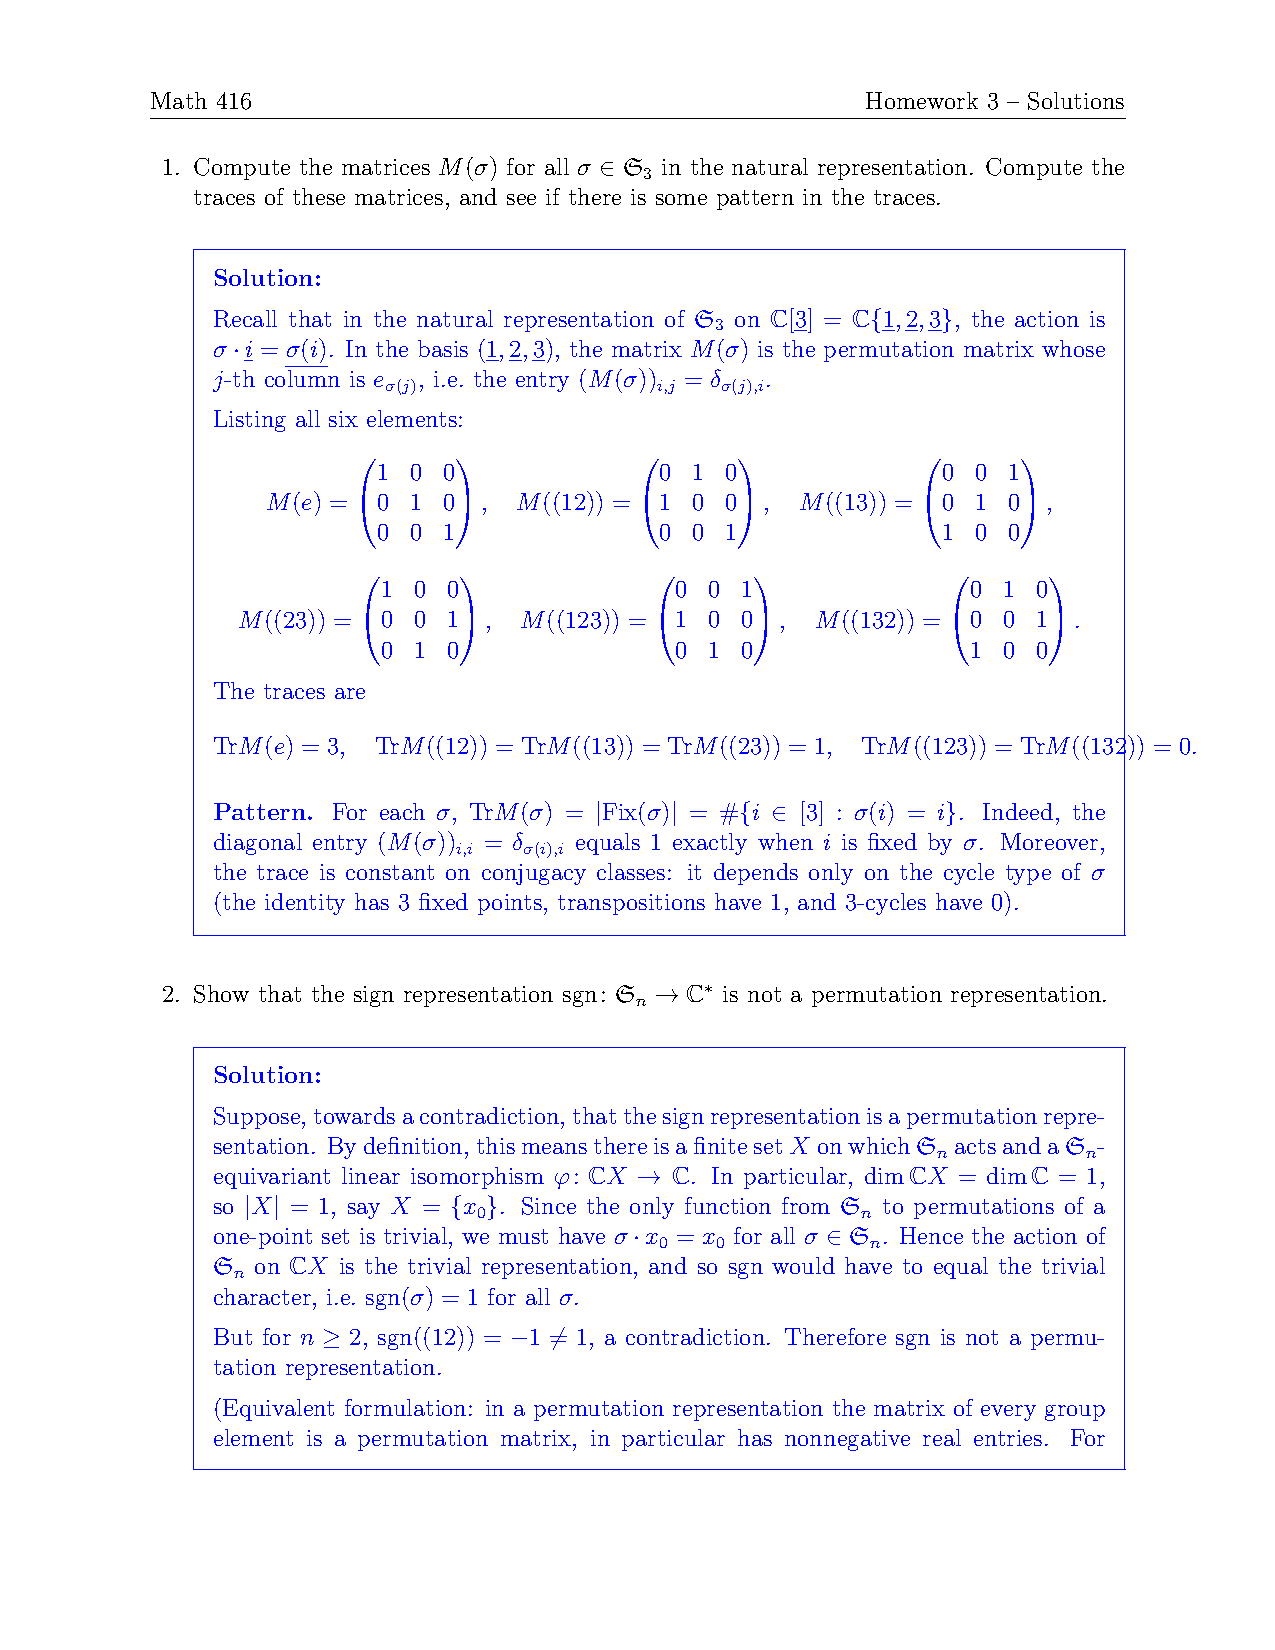
\includepdf[pages=-]{pdfs/HWK3-solutions.pdf}

\section{Test 2 Review}

\subsection{Theorems and Proofs of Theorems}

\begin{myboxg}
    \begin{lemma}[Lemma 3.2]
        If $X$ is a $G$-set, then $G_{gx} = g G_x g^{-1}$ for any $g \in G$ and $x \in X$.
    \end{lemma}
\end{myboxg}

\begin{proof}
    An element $u \in G$ stabilizes $gx$ if and only if $g^{-1} u g$ stabilizes $x$, 
    which occurs if and only if $u \in g G_x g^{-1}$.
\end{proof}

\begin{myboxg}
    \begin{proposition}[Proposition 3.4]
        If $X$ is a transitive $G$-set, then $X \cong G / G_x$ as $G$-sets for any $x \in X$.
    \end{proposition}
\end{myboxg}

\begin{proof}
    Let $x \in X$, and define $\varphi : G / G_x \to X$ by $\varphi(gG_x) = gx$ for $g \in G$.  
    
    If $gG_x = g'G_x$ for $g, g' \in G$, then $g^{-1}g' \in G_x$ and hence
    $g^{-1}g' x = x$, giving $gx = g'x$. This shows that $\varphi$ is well-defined.  
    By reversing the argument, we see that $\varphi$ is injective.
    
    For any $u \in G$ and $gG_x \in G / G_x$, we have
    \[
    u \varphi(gG_x) = u(gx) = (ug)x = \varphi(ugG_x) = \varphi(u(gG_x)),
    \]
    showing that $\varphi$ is a $G$-set homomorphism.
    
    For any $y \in X$, by transitivity there exists some $g \in G$ such that
    $y = gx = \varphi(gG_x)$, so $\varphi$ is surjective.
    
    Therefore, $\varphi$ is a $G$-set isomorphism.
\end{proof}

\begin{myboxg}
    \begin{lemma}[Lemma 3.6]
        Let $\varphi : X \to Y$ be a homomorphism of $G$-sets, and let $x \in X$. 
        Then $G_x \leqslant G_{\varphi(x)}$, and if $\varphi$ is an isomorphism, then 
        $G_x = G_{\varphi(x)}$.
    \end{lemma}
\end{myboxg}

\begin{proof}
    If $g \in G_x$, then $\varphi(x) = \varphi(gx) = g\varphi(x)$; it follows that 
    $g \in G_{\varphi(x)}$. Hence $G_x \leqslant G_{\varphi(x)}$.
    
    If $\varphi$ is an isomorphism, then by considering the $G$-set homomorphism 
    $\varphi^{-1} : Y \to X$, we have
    \[
    G_{\varphi(x)} \leqslant G_{\varphi^{-1}(\varphi(x))} = G_x.
    \]
    Therefore, $G_x = G_{\varphi(x)}$.
\end{proof}

\begin{myboxg}
    \begin{corollary}[Corollary 3.5]
        Let $X$ be a $G$-set. Then $Gx \cong G / G_x$ as $G$-sets for any $x \in X$. 
        In particular, if $G$ is finite, then $|Gx| = [G : G_x]$.
    \end{corollary}
\end{myboxg}

\begin{myboxg}
    \begin{proposition}[Proposition 3.3]
        Any $G$-set has a unique partition consisting of transitive $G$-sets, 
        namely its partition into orbits.
    \end{proposition}
\end{myboxg}

\begin{proof}
    First, note that if $X$ has a partition consisting of transitive $G$-sets, 
    then those sets must be the orbits, since the orbits are precisely the 
    transitive subsets of $X$. This proves uniqueness.
    
    For existence, let $x \in X$. Then $x$ lies in the orbit $Gx$, so it suffices 
    to show that any two orbits of $X$ under the action of $G$ are either equal 
    or disjoint.
    
    Let $x, y \in X$ and suppose that $Gx \cap Gy$ is non-empty. Then there exist 
    $g_1, g_2 \in G$ such that
    \[
    g_1 x = g_2 y.
    \]
    It follows that
    \[
    y = g_2^{-1} g_1 x \in Gx,
    \]
    and hence $Gy \subseteq Gx$. By symmetry, we also have $Gx \subseteq Gy$, 
    and therefore $Gx = Gy$.
\end{proof}

\begin{myboxg}
    \begin{theorem}[Cayley's Theorem]
        Every group $G$ is isomorphic to a subgroup of $\operatorname{Sym}(G)$. 
        In particular, if $G$ is finite with $|G| = n$, then $G$ is isomorphic 
        to a subgroup of $\operatorname{Sym}(n)$.
    \end{theorem}
\end{myboxg}

\begin{proof}
    The group $G$ acts on itself by left multiplication, i.e., for $g,x \in G$,
    define $g \cdot x = gx$. This is the case $H = \{1\}$ of the action of $G$ 
    on the coset space $G/H$.
    
    If $g \in G$ satisfies $gx = x$ for all $x \in G$, then taking $x = g^{-1}$ 
    gives $g^{-1} = gg^{-1} = 1$, and hence $g = 1$. Therefore, the action is 
    faithful.
    
    Thus, we obtain an injective homomorphism (a monomorphism) from $G$ into 
    $\operatorname{Sym}(G)$, and the result follows.
\end{proof}

\begin{myboxg}
    \begin{theorem}[Sylow's Theorem]
        Let $G$ be a finite group and let $p$ be a prime dividing $|G|$. Then the following hold:
        \begin{enumerate}
            \item $G$ has at least one Sylow $p$-subgroup.
            \item All Sylow $p$-subgroups of $G$ are conjugate.
            \item Any $p$-subgroup of $G$ is contained in a Sylow $p$-subgroup.
            \item The number of Sylow $p$-subgroups of $G$ is congruent to $1 \pmod{p}$.
        \end{enumerate}
    \end{theorem}
\end{myboxg}

\begin{myboxg}
    \begin{theorem}[Sylow's Theorem's Alternative]
        Let $p$ be prime and $G$ a group of order $|G|= p^am$m, and $\textnormal{gcd}(p^a,m)=1$. Then
        \begin{enumerate}[(1)]
            \item Every $p-$subgroup is contained in a Sylow $p-$subgroup . In particular, Sylow subgroups exist.
            \item If $n_p$ is the number of Sylow $p-$subgroups, then $n_p \equiv 1 (\textnormal{mod}p)$
            \item $n_p|m$ 
            \item all Sylow $p-$subgroups are conjugate of each other
        \end{enumerate}
    \end{theorem}
\end{myboxg}

\begin{myboxg}
    \begin{theorem}[Cauchy's Theorem]
        Let $G$ be a finite group and let $p$ be a prime dividing $|G|$. 
        Then $G$ has an element of order $p$.
    \end{theorem}
\end{myboxg}

\begin{proof}
    By part (i) of Sylow's Theorem, $G$ has a nontrivial Sylow $p$-subgroup. 
    Hence $G$ contains a nontrivial $p$-element, some power of which has order $p$.
\end{proof}

\begin{myboxg}
    \begin{theorem}[$p<q$ Theorem]
        Let $p,q $ be two primes with $p< q$ and $|G|=pq$. Then $G$ has only one $q-$subgroup and so this $q-$subgroup is normal. Additionally, whenever $q \not \equiv 1 \mod p$, then there is a unique group of order $pq$ which is $\mathbb{Z}_{pq}$
    \end{theorem}
\end{myboxg}

\begin{proof}
    From Sylow's theorem we know that $n_q|p$, and $n_p \equiv 1\mod p$. This tells us that $n_q = 1, 1+q, 1+2q, \cdots $. However, $1 +kq >p$ for $k>0$. So it must be the case the $n_q = 1$. Let $Q$ be this Sylow $q-$subgroup. This means that $Q \triangleleft G$. Similarly, from Sylow's theorem, we know that $n_p|q$, and $n_p \equiv 1 \mod p$. This means $n_p =1, 1+p, 1+2p, \cdots$. If $q \not \equiv 1 \mod p$, then $n_p = 1$. Let $P$ be this Sylow $p-$subgroup. Since $n_p =1$, we know that $P \triangleleft G$
    \vspace{10pt}
    We know that $P \cap Q = \{ e \}$ since each groups are of prime order; meaning they are both cyclic and generated by differing elements. Now that we know both $P$ and $Q$ are normal, we see that the internal direct product $PQ=QP \leqslant G$. The statement $P\cap Q = \{ e \}$ and $PQ = QP \leqslant G$ show that $|PQ|=|QP|=pq = |G|$. Hence $PQ = G$. Furthermore, we see that $G = PQ \cong P \times Q$. Since both $P$ and $Q$ are cyclic groups of prime order $P \cong \mathbb{Z}_p$ and $Q \cong \mathbb{Z}_q$, thus $G \cong P \times Q \cong \mathbb{Z}_p \times \mathbb{Z}_q \cong \mathbb{Z}_{pq}$.
\end{proof}

\begin{myboxg}
    \begin{theorem}[Theorem 8.1]
        If $P$ is a nontrivial finite $p$-group, then $Z(P)$ is also nontrivial. 
        Moreover, if $N \neq \{1\}$ is a normal subgroup of $P$, then 
        $N \cap Z(P) \neq \{1\}$.
    \end{theorem}
\end{myboxg}

\begin{proof}
    Suppose that $Z(P) = \{1\}$. Let $K_1 = \{1\}, K_2, \dots, K_r$ be the conjugacy classes of $P$. 
    If $K_i = \{x\}$ for some $i$ and some $x \in P$, then $gxg^{-1} = x$ for all $g \in P$, 
    which shows that $x \in Z(P) = \{1\}$. Therefore, $|K_i| > 1$ for each $1 <i \leq r$.
    
    Each $K_i$ is an orbit under the action of $P$ on itself by conjugation, so $|K_i|$ divides $|P|$ 
    for all $i$. Since $P$ is a $p$-group, it follows that $|K_i| \equiv 0 \pmod{p}$ for each $1 <i \leq r$.
    
    Now,
    \[
    |P| = |K_1| + |K_2| + \cdots + |K_r| = 1 + |K_2| + \cdots + |K_r| \equiv 1 \pmod{p},
    \]
    since $P$ is the disjoint union of $K_1, \cdots, K_r$. This is a contradiction, since $|P|$ is divisible by $p$. Therefore, $Z(P)$ is nontrivial.
    
    Now let $N \trianglelefteq P$ with $N \neq \{1\}$. Then $N$ is a union of some of the conjugacy 
    classes $K_j$, where the index set $S \subseteq \{1, \dots, r\}$ contains $1$ and $|S| > 1$. 
    If $N \cap Z(P) = \{1\}$, then $|K_j| > 1$ for all $j \in S$ with $j \neq 1$, and as above 
    this would imply
    \[
    |N| \equiv 1 \pmod{p},
    \]
    which is impossible since $|N|$ is divisible by $p$. Therefore, 
    $N \cap Z(P) \neq \{1\}$.
\end{proof}

\begin{myboxg}
    \begin{lemma}[Lemma 8.2]
        If $G$ is a non-abelian group, then $G/Z(G)$ cannot be cyclic. 
        In particular, if $P$ is a finite $p$-group, then $[P : Z(P)] \neq p$.
    \end{lemma}
\end{myboxg}

\begin{proof}
    Suppose that $G/Z(G) = \langle xZ(G) \rangle$ for some $x \in G$. 
    Then $G$ is generated by the set $S = Z(G) \cup \{x\}$.
    
    Every pair of elements in $S$ commutes: elements of $Z(G)$ commute with all elements of $G$, 
    and hence with $x$, while elements of $Z(G)$ commute with each other. Therefore, all elements 
    of $S$ commute, and it follows that $\langle S \rangle = G$ is abelian, a contradiction.
    
    For the second statement, if $P$ is a finite $p$-group and $[P : Z(P)] = p$, then 
    $P/Z(P)$ has order $p$ and is therefore cyclic, contradicting the first part. 
\end{proof}

\begin{myboxg}
    \begin{theorem}[Theorem 8.7]
    The following statements about a finite group $G$ are equivalent:
        \begin{enumerate}
            \item Every Sylow subgroup of $G$ is normal in $G$.
            \item $G$ is the direct product of its Sylow subgroups.
            \item Every maximal subgroup of $G$ is normal in $G$.
        \end{enumerate}
    \end{theorem}
\end{myboxg}

\begin{myboxg}
    \begin{proposition}[Proposition 10.1]
        Finite groups have composition series.
    \end{proposition}
\end{myboxg}

\begin{proof}
    Let $G$ be a finite group. We proceed by induction on $|G|$.
    
    If $G$ is simple, then $G > \{1\}$ is a composition series of $G$.
    
    Otherwise, $G$ has a maximal normal subgroup $G_1$, which by induction 
    has a composition series
    \[
    G_1 > G_2 > \cdots > G_r = \{1\}.
    \]
    Since $G/G_1$ is simple, it follows that
    \[
    G = G_0 > G_1 > \cdots > G_r = \{1\}
    \]
    is a composition series of $G$.
\end{proof}

\begin{myboxg}
    \begin{lemma}[Lemma 10.2]
        Let $G$ be a group that has a composition series, and let $N \trianglelefteq G$. 
        Then $N$ has a composition series.
    \end{lemma}
\end{myboxg}

\begin{myboxg}
    \begin{theorem}[Jordan--Hölder Theorem]
        Suppose that $G$ is a group that has a composition series. Then any two 
        composition series of $G$ have the same length and are equivalent.
    \end{theorem}
\end{myboxg}

\subsection{Important Definitions for Test 2}

\begin{definition}
    Let $G$ be a group $|G| = p^am$, and $\textnormal{gcd}(p^a,m)=1$. A $p$-subgroup is a subgroup $H \leqslant G$ with $|H|=p^k$ for $k \leq a$. If $k = a$ we call it a Sylow $p-$subgroup.
\end{definition}

\begin{theorem}[The Structure of Finite Abelian $p-$Groups]
    Every finite abelian $p-$group is isomorphic to a direct product
    \begin{align}
        G \cong \mathbb{Z}_{p^{a_1}} \times \cdots \times \mathbb{Z}_{p^{a_k}}
    \end{align}
\end{theorem}

\begin{theorem}[Fundamental Theorem of Finite Abelian Groups]
    Every finite abelian group is uniquely isomorphic to $G = \mathbb{Z}_{q_1^{a_1}} \times \cdots \times \mathbb{Z}_{q_r^{a_r}}$. Where $q_r$ are (not necessarily distinct) primes. 
\end{theorem}

\begin{lemma}
    Every finite abelian group is isomorphic to the product of its Sylow subgroups, that is if $|G| =p_1^{a_1}\cdots p_k^{a_k}$ and $P_i$ is the unique Sylow $P_i-$subgroup, then $G \cong P_1 \times P_2 \times \cdots \times P_k$
\end{lemma}

\begin{definition}[Subnormal Series]
    A subnormal series of $G$ is a chain
    \begin{align}
        \{ e \} = G_0 \trianglelefteq G_1 \trianglelefteq G_2 \trianglelefteq G_3 \trianglelefteq \cdots \trianglelefteq G_n = G 
    \end{align}
\end{definition}

\begin{definition}[The Factors of A Series]
    The quotients $\sfrac{G_{i +1}}{G_i}$ are the factors of the series.
\end{definition}

\begin{definition}[A Composition Series of $G$]
    A composition series of $G$ is a subnormal series:
    \begin{align}
        \{ e \} \triangleleft G_1 \triangleleft G_2 \triangleleft \cdots \triangleleft G_n = G
    \end{align}
    here $\sfrac{G_{i+1}}{G_i}$ is a \textit{simple group}. This means that $\sfrac{G_{i+1}}{G_i}$ has no proper normal subgroups.
\end{definition}

\begin{example}
    Let $\sfrac{\mathbb{Z}}{12 \mathbb{Z}}$ We can see the composition series of this becomes
    \begin{align}
        \{ 0 \}\triangleleft \langle 6 \rangle \triangleleft \langle 3 \rangle \triangleleft \langle 1 \rangle = \sfrac{\mathbb{Z}}{12 \mathbb{Z}}
    \end{align}
    We can look at some of the factors of the composition series
    \begin{align}
        \sfrac{\langle 6 \rangle}{ \langle 0 \rangle} & \cong \sfrac{\mathbb{Z}}{2 \mathbb{Z}} \\
        \sfrac{\langle 3 \rangle}{\langle 6 \rangle} &\cong \sfrac{\mathbb{Z}}{2 \mathbb{Z}} \\
        \sfrac{\langle 1 \rangle}{\langle 3 \rangle} &\cong \sfrac{\mathbb{Z}}{3\mathbb{Z}}
    \end{align}
\end{example}

\subsection{Alternative Answers For Test 2}

\begin{problem}[QUESTION 1]
    This problem is divided into several parts:
    \begin{enumerate}[(a)]
            \item Let $X$ and $Y$ be $G$-sets. A \textbf{$G$-set isomorphism} is a bijection $\phi: X \to Y$ such that
            \begin{align}
                \phi(g \cdot x) = g \cdot \phi(x)
            \end{align}
            for all $g \in G$ and $x \in X$.
            \item ---(his solution is good)---
            \item ---(his solution is good)---
            \item ---(his solution is good)---
            \item ---(his solution is good)---
            \item ---(his solution is good)---
            \item ---(his solution is good)---
    \end{enumerate}
\end{problem}

\begin{problem}[QUESTION 2]
    An element $u \in G$ stabilizes $gx$ if and only if $g^{-1} u g$ stabilizes $x$, 
    which occurs if and only if $u \in g G_x g^{-1}$.
\end{problem}

\begin{problem}[QUESTION 3]
    Let $x \in X$, and define $\varphi : G / G_x \to X$ by $\varphi(gG_x) = gx$ for $g \in G$.  
    
    If $gG_x = g'G_x$ for $g, g' \in G$, then $g^{-1}g' \in G_x$ and hence
    $g^{-1}g' x = x$, giving $gx = g'x$. This shows that $\varphi$ is well-defined.  
    By reversing the argument, we see that $\varphi$ is injective.
    
    For any $u \in G$ and $gG_x \in G / G_x$, we have
    \[
    u \varphi(gG_x) = u(gx) = (ug)x = \varphi(ugG_x) = \varphi(u(gG_x)),
    \]
    showing that $\varphi$ is a $G$-set homomorphism.
    
    For any $y \in X$, by transitivity there exists some $g \in G$ such that
    $y = gx = \varphi(gG_x)$, so $\varphi$ is surjective.
    
    Therefore, $\varphi$ is a $G$-set isomorphism.
\end{problem}

\begin{problem}[QUESTION 4]
    Recall that if we let $G$ be a group $|G| = p^am$, and $\textnormal{gcd}(p^a,m)=1$. A $p$-subgroup is a subgroup $H \leqslant G$ with $|P|=p^k$ for $k \leq a$. If $k = a$ we call it a Sylow $p-$subgroup. Our goal is to show that if for $k = a$, $H \trianglelefteq G$, and $|P|=p^a$, then $H \subseteq P$. We can start off by seeing $H$ as a $p-$group where $k=1$, since we let $|H|=p$, from Sylow's theorem we know that $H\subseteq P'$ for some Sylow $p-$subgroup $P'$. Since $H \trianglelefteq G$, $g H g^{-1}=H$, $H =gHg^{-1} \subseteq gP'g^{-1}$ for some $g \in G$. However, because all Sylow $p-$subgroups are conjugate of one another, $gP'g^{-1} = P$, where $P$ is any arbitrary Sylow $p-$subgroup. So $H \subseteq P$.
\end{problem}

\begin{problem}[QUESTION 5]
    We will begin by decomposing the order of $G$. We can see that $|G|=5\cdot 8 = 40$. From Sylow's theorem, we know that the number of Sylow $5-$subgroups, $n_5 \equiv 1 \mod 5$, and that $n_5|8$. With this in mind the only divisors of $8$ that are congruent to $1$, so $n_5 = 1$. Since the subgroup is unique it must be normal. This tells us that all groups of order $40$ are not simple as they have at least one normal subgroup of order $5$. 
\end{problem}

\begin{problem}[QUESTION 6]
    Base Case:  If $|G|=2$, then $G \cong \sfrac{\mathbb{Z}}{2 \mathbb{Z}}$ is simple, and $\{ e \} \triangleleft G$ is a composition series.
    
    \vspace{10pt}

    Inductive Step: Assume that ever group of order less than $|G|$ has a composition series.
    \begin{itemize}
        \item If $G$ is a simple group, then $\{ e \} \triangleleft G$ is a composition series (we are done). 
        \item If $G$ is not simple, then $G$ has a proper nontrivial normal subgroup. Among all of those subgroups, choose $N$ to be the maximal proper normal subgroup of $G$. From this we know that $\sfrac{G}{N}$ is simple because Any normal subgroup of $\sfrac{G}{N}$ would correspond to a normal subgroup of $G$ containing $N$. By maximality, this must be $\sfrac{G}{N}$ itself or it is trivial. Since $|N| < |G|$, by the induction hypothesis, $N$ has a composition series:
        \begin{align}
            \{ e \} = N_0 \triangleleft N_1 \triangleleft \cdots N_k = N
        \end{align}
    \end{itemize}
    Then: 
    \begin{align}
        \{ e \} = N_0 \triangleleft N_1 \triangleleft \cdots N_k = N \triangleleft G
    \end{align}
    Because every factor $\sfrac{N_{i+1}}{N_i}$ is simple and $\sfrac{G}{N}$ is simple 
\end{problem}

\begin{problem}[QUESTION 7]
    If we look at the conjugation action $G^{\circlearrowright^G}$ with $\mathrm{Fix}(G)= Z(G)$, by the class equation we know 
    \begin{align}
        |G| = |\mathrm{Fix}(G)| + \sum_{h \in G} [G:G_h].
    \end{align}
    We also know that $|G|$ needs to be divided by each $[G:G_h]$. So we must have $[G:G_h]||G|=p^a$; hence, we require $p|[G:G_h]$. So our class equation is now
    \begin{align}
        |G|= p^a = |Z(G)| + p^{b_1}+\cdots + p^{b_n},
    \end{align}
    where $b_i < a$. So it must be the case that $p||Z(G)|$, meaning $Z(G)$ is nontrivial.
\end{problem}

\begin{problem}[QUESTION 8]
    Suppose we let $G$ be an abelian group of order $m$ and have $n | m$. We will show that $G$ has a subgroup of order $n$. We can consider the prime factorizations of $n$ and $m$:
    \begin{align}
        \prod_{i = 1}^{r}p_i^{a_1} = m, \quad \prod_{i = 1}^{r}p_i^{b_i} = n
    \end{align}
    where $0 \leq b_i \leq a_i$ for $i = 1, 2, \cdots, r$. Since we know that $G$ is a finite abelian group, it is the direct product of Sylow $p_i-$subgroups:
    \begin{align}
        G \cong G_{p_1} \times G_{p_2} \times \cdots \times G_{p_r}
    \end{align}
    where each $G_{p_i}$ is an abelian $p_i-$group of order $p_i^{a_i}$. So it is enough to show that if $P$ is a finite abelian group of order $p^a$, then for any $0 \leq b \leq a$, there exists a subgroup $H$ of order $b$ in $P$. This is true since we can represent a subgroup of order $n$ of $G$ by a direct product of $p_i-$subgroups that match the structure of the prime factorization of $n$. For example if $H_i \leq G_{p_i}$ where $|H_i| = p_{i}^{b_i}$, then 
    \begin{align}
        H_1 \times H_2 \times \cdots \times H_r \leq G
    \end{align}
    has order $\prod_{i = 1}^{r}p_i^{b_i} = n$.
    Now if we let $P$ be a finite abelian group of order $p^a$, the fundamental theorem of finite abelian groups tells us that
    \begin{align}
        P \cong \mathbb{Z}_{p^{e_1}} \times \mathbb{Z}_{p^{e_2}}  \times \cdots \times \mathbb{Z}_{p^{e_t}}
    \end{align}
    where $e_1 + e_2 + \cdots + e_t = a$. For each of the $\mathbb{Z}_{p^{e_i}}$ there is a subgroup of order $\mathbb{Z}_{p^{c_i}}$. For each of these groups in the direct product we can adjust each $c_i$ to get $c_1 + c_2 + \cdots +c_t = b$. The corresponding direct product of subgroups will be of order $p^{c_1}\cdot p^{c_2}\cdots p^{c_t}= p^b$. Hence $P$ has a subgroup of order $p^b$.
\end{problem}

\subsection{Test 2 Solutions}

% Inserting a PDF
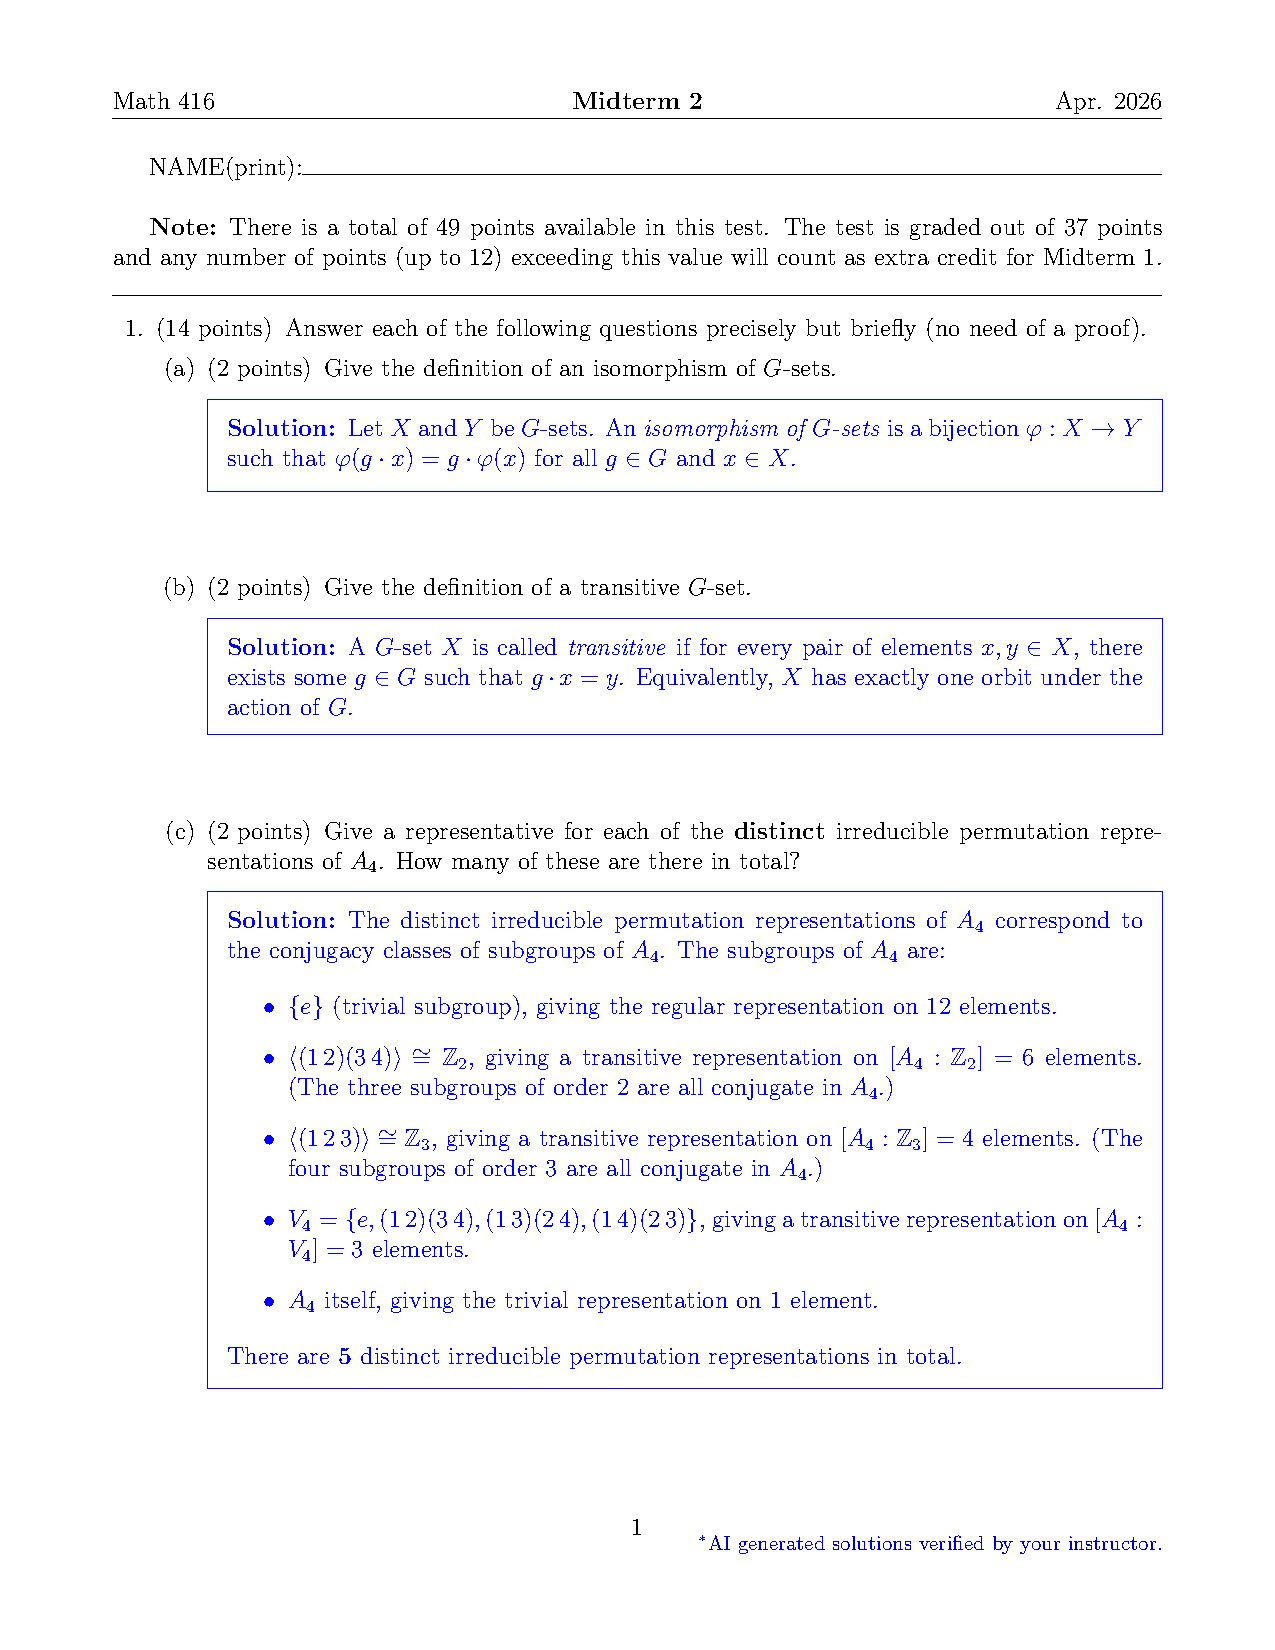
\includepdf[pages=-]{pdfs/midterm_2-MATH416-solutions.pdf}

\section{Test 1 Review}

\subsection{Alternative Answers for Test 1}

\begin{problem}[QUESTION 1]
    The answers are enumerated as follows:
    \begin{enumerate}[(a)]
        \item Let $f: H \to G$ be a homomorphism. Then we know that $\mathrm{Ker}f \triangleleft H, \mathrm{Im}f \leqslant G$, and $\sfrac{H}{\mathrm{Ker}f} \cong \mathrm{Im}f$
        \item ---(His Solution is Good)---
        \item ---(His Solution is Good)---
        \item ---(His Solution is Good)---
        \item ---(His Solution is Good)---
        \item ---(His Solution is Good)---
    \end{enumerate}
\end{problem}

\begin{problem}[QUESTION 2]
    Since $\mathcal{C}$ is a family of subsets of $G$ that form a partition of $G$, we know $\exists C \in \mathcal{C}$ where $e\in C$. We will show that this particular $C$ is a subgroup of $G$. Suppose $G$ is of the form $G = \{ e,x_1,x_2, \cdots, x_{n-2}, x_{n-1} \}$ where $n$ is the order of the group.
    \begin{enumerate}
        \item \textbf{Existence of Identity:} By construction we know that $e \in C$.
        \item \textbf{Closure Under Inverses:} Take any $x_i \in C$. If we observe $x_iC$ we see that $x_i \in x_iC$ since $e \in C$ and $x_i=x_i e \in x_iC$. However, since $x_1C \in \mathcal{C}$, meaning $x_iC$ is a partition, and $x_i \in x_iC$, it must be the case that $x_iC = C$. From this we know that $e \in x_iC$ since $x_iC = C$, or, in other words, $e = x_i x_j$ for some $x_j \in C$. The only element in $G$ that can satisfy this is $x_i^{-1}$. Here we can conclude that $x_i^{-1} \in C$.
        \item \textbf{Closure Under Operations:} Take $x_i, x_j \in C$. We see that $x_j x_i \in x_jC$. However, we showed for any $x_j \in C$, $x_j C = C$. So $x_jx_i \in C = x_jC$.
    \end{enumerate}
    Now we will show that $\mathcal{C}$ is a set of cosets of $C$ in $G$, or $\mathcal{C} = G/C$. We will first observe the definition of the set $G/C$
    \begin{align}
        G/C = \{ gC | g \in G \}
    \end{align}
    From the premise, we know that $gC \in \mathcal{C} \quad \forall g \in G$. With this and the definition of $G/C$, we see that $G/C \subseteq \mathcal{C}$. Furthermore, we can take any random partition $D \in \mathcal{C}$. If we take some element $x_k \in D$, we see $e\in x_k^{-1}D$ since $e = x_k^{-1}x_k \in x_k^{-1}D$. This means $x_k^{-1}D = C$. If we left multiply by $x_k$ we get $D = x_kx_k^{-1}D= x_kC$. Since $x_k \in G$, $D=x_kC\in G/C$, or $\mathcal{C}\subseteq G/C$
\end{problem}

\begin{problem}[QUESTION 3]
    We take $\sigma \in \mathrm{Aut}(G)$ and $\varphi_g \in \mathrm{Inn}(G)$ for some $g \in G$. We observe if we have $\sigma \varphi_g\sigma^{-1}(x)$ for $x \in G$
    \begin{align}
        \sigma \varphi_g\sigma^{-1}(x) = \sigma (g\sigma^{-1}(x)g^{-1})= \sigma(g)\sigma(\sigma^{-1}(x))\sigma^{-1}(g) = \sigma(g)x\sigma^{-1}(g) = \varphi_{\sigma(g)}(x).
    \end{align}
    Hence $\varphi_g(x) \in \mathrm{Inn}(G)$, implying that $\sigma \mathrm{Inn}(G)\sigma^{-1} \subseteq \mathrm{Inn}(G)$. This shows that $\mathrm{Inn}(G) \triangleleft \mathrm{Aut}(G)$.
\end{problem}

\begin{problem}[QUESTION 4]
    Let $\sigma : G \to \mathfrak{S}_{\sfrac{G}{H}} \cong \mathfrak{S}_p$ defined by $g \mapsto \sigma(g)(x) = gxH, x\in G$. This means that $\sigma$ is a homomorphism. From this, we can see that:
    \begin{align}
        \mathrm{Ker}(\sigma) &= \{ g \in G | gxH = xH, \forall x \in G \} \\
        &= \{ g \in G | x^{-1}gxH = H, \forall x \in G \} \\
        &= \{ g \in G | x^{-1}gx \in H, \forall x \in G \} \\
        &= \{ g \in G | g \in x^{-1}Hx, \forall x \in G \} \\
        &= \bigcap_{x \in G} x^{-1}H x \leqslant H,
    \end{align}
    since the intersection of subgroups is always a subgroup. Furthermore, by the first isomorphism theorem we know that $\sfrac{G}{\mathrm{Ker}(\sigma)} \cong \mathrm{Im}(\sigma) \implies |\sfrac{G}{\mathrm{Ker}(\sigma)}| = |\mathrm{Im}(\sigma)|||\mathfrak S_{p}| = p!$. But we know that $|\sfrac{G}{\mathrm{Ker}(\sigma)}|= |\sfrac{G}{H}|\cdot |\sfrac{H}{\mathrm{Ker}(\sigma)}| = p \cdot |\sfrac{K}{\mathrm{Ker}(\sigma)}|$. From here we can observe that $p \cdot |\sfrac{K}{\mathrm{Ker}(\sigma)}||p! == p \cdot (p-1)! \implies |\sfrac{K}{\mathrm{Ker}(\sigma)}| | (p-1)!$. We also see that since $\mathrm{Ker}(\sigma) \leqslant H$, this implies that $|\sfrac{H}{\mathrm{Ker}(\sigma)}||H|$, but all primes that divide $H$ are greater than or equal to $p$ since $\frac{|G|}{|H|}= p$. So all primes that divide $|\sfrac{H}{\mathrm{Ker}(\sigma)}|$ are greater than $p$. Since $|\sfrac{H}{\mathrm{Ker}(\sigma)}||(p-1)!$, this means that $|\sfrac{H}{\mathrm{Ker}(\sigma)}|=1$. This implies that $H = \mathrm{Ker}(\sigma) \triangleleft G$ since the kernel is always normal in $G$ for a homomorphism.
\end{problem}

\begin{problem}[QUESTION 5]
    We must show that $G \cong H \leqslant \mathfrak{S}_G$. Let $\sigma : G \to \mathfrak{S}_G$ be a left permutation representation defined by $g \mapsto \sigma(g)(x) = g \cdot x$ for $x, g \in G$. From this, $\sigma$ is readily seen as a homomorphism
    \begin{align}
        \sigma(gh)(x) = gh \cdot x = g \cdot (h \cdot x) = \sigma(g)(\sigma(h)(x)) = \sigma(g) \circ \sigma(h)(x).
    \end{align}
    By the first isomorphism theorem, we know that $\sfrac{G}{\mathrm{Ker}(\sigma)} \cong \mathrm{Im}(\sigma)$. Since $\sigma$ is a homomorphism, $\mathrm{Ker}(\sigma) = \{ e \}$ and $\mathrm{Im}(\sigma) \leqslant \mathfrak{S}_G$. So we can see $G \cong \sfrac{G}{\{e\}} \cong \mathrm{Im}(\sigma) \leqslant \mathfrak{S}_G$
\end{problem}

\begin{problem}[QUESTION 6]
    ---(HIS SOLUTION IS GOOD)---
\end{problem}

\subsection{Test 1 Solutions}

% Inserting a PDF
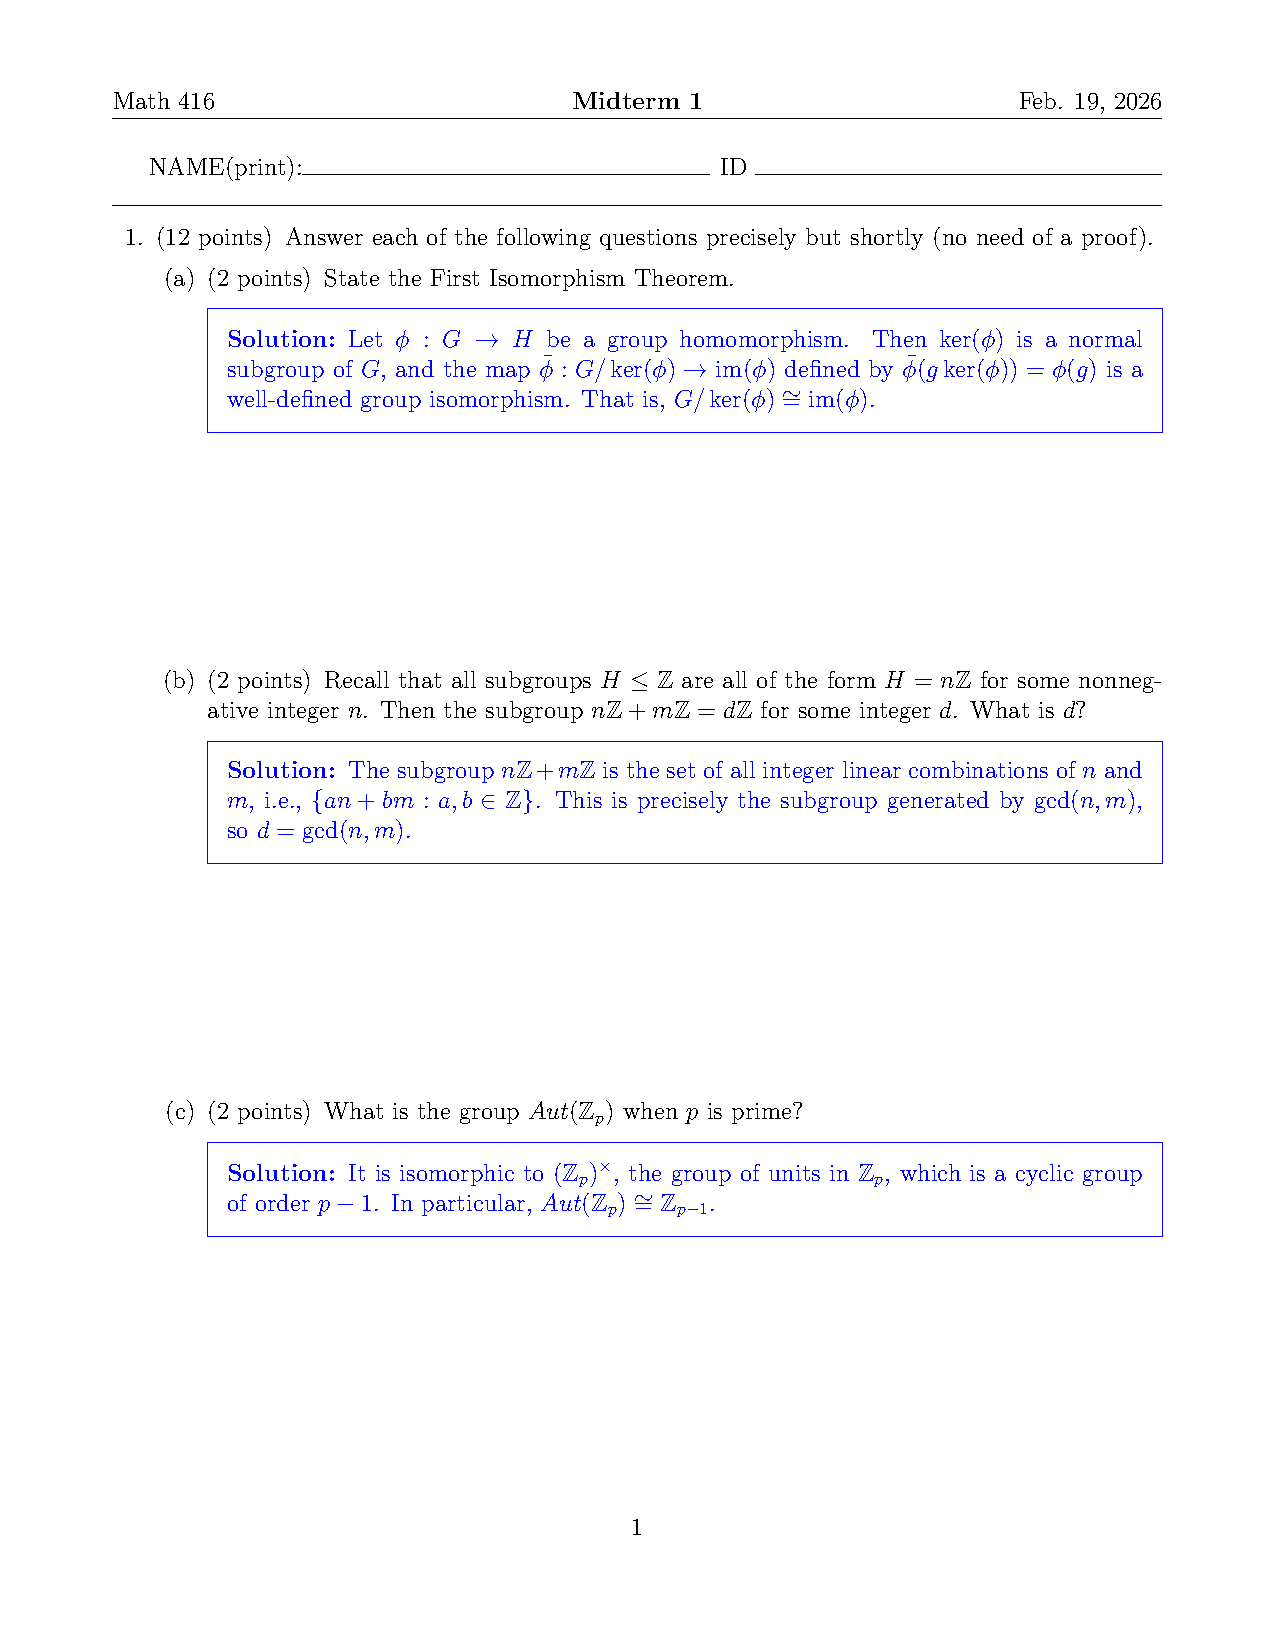
\includepdf[pages=-]{pdfs/midterm_1-MATH416-solutions.pdf}

\end{document}

